% Options for packages loaded elsewhere
\PassOptionsToPackage{unicode}{hyperref}
\PassOptionsToPackage{hyphens}{url}
%
\documentclass[
]{article}
\title{Vaccination}
\author{FD}
\date{}

\usepackage{amsmath,amssymb}
\usepackage{lmodern}
\usepackage{iftex}
\ifPDFTeX
  \usepackage[T1]{fontenc}
  \usepackage[utf8]{inputenc}
  \usepackage{textcomp} % provide euro and other symbols
\else % if luatex or xetex
  \usepackage{unicode-math}
  \defaultfontfeatures{Scale=MatchLowercase}
  \defaultfontfeatures[\rmfamily]{Ligatures=TeX,Scale=1}
\fi
% Use upquote if available, for straight quotes in verbatim environments
\IfFileExists{upquote.sty}{\usepackage{upquote}}{}
\IfFileExists{microtype.sty}{% use microtype if available
  \usepackage[]{microtype}
  \UseMicrotypeSet[protrusion]{basicmath} % disable protrusion for tt fonts
}{}
\makeatletter
\@ifundefined{KOMAClassName}{% if non-KOMA class
  \IfFileExists{parskip.sty}{%
    \usepackage{parskip}
  }{% else
    \setlength{\parindent}{0pt}
    \setlength{\parskip}{6pt plus 2pt minus 1pt}}
}{% if KOMA class
  \KOMAoptions{parskip=half}}
\makeatother
\usepackage{xcolor}
\IfFileExists{xurl.sty}{\usepackage{xurl}}{} % add URL line breaks if available
\IfFileExists{bookmark.sty}{\usepackage{bookmark}}{\usepackage{hyperref}}
\hypersetup{
  pdftitle={Vaccination},
  pdfauthor={FD},
  hidelinks,
  pdfcreator={LaTeX via pandoc}}
\urlstyle{same} % disable monospaced font for URLs
\usepackage[margin=1in]{geometry}
\usepackage{color}
\usepackage{fancyvrb}
\newcommand{\VerbBar}{|}
\newcommand{\VERB}{\Verb[commandchars=\\\{\}]}
\DefineVerbatimEnvironment{Highlighting}{Verbatim}{commandchars=\\\{\}}
% Add ',fontsize=\small' for more characters per line
\usepackage{framed}
\definecolor{shadecolor}{RGB}{248,248,248}
\newenvironment{Shaded}{\begin{snugshade}}{\end{snugshade}}
\newcommand{\AlertTok}[1]{\textcolor[rgb]{0.94,0.16,0.16}{#1}}
\newcommand{\AnnotationTok}[1]{\textcolor[rgb]{0.56,0.35,0.01}{\textbf{\textit{#1}}}}
\newcommand{\AttributeTok}[1]{\textcolor[rgb]{0.77,0.63,0.00}{#1}}
\newcommand{\BaseNTok}[1]{\textcolor[rgb]{0.00,0.00,0.81}{#1}}
\newcommand{\BuiltInTok}[1]{#1}
\newcommand{\CharTok}[1]{\textcolor[rgb]{0.31,0.60,0.02}{#1}}
\newcommand{\CommentTok}[1]{\textcolor[rgb]{0.56,0.35,0.01}{\textit{#1}}}
\newcommand{\CommentVarTok}[1]{\textcolor[rgb]{0.56,0.35,0.01}{\textbf{\textit{#1}}}}
\newcommand{\ConstantTok}[1]{\textcolor[rgb]{0.00,0.00,0.00}{#1}}
\newcommand{\ControlFlowTok}[1]{\textcolor[rgb]{0.13,0.29,0.53}{\textbf{#1}}}
\newcommand{\DataTypeTok}[1]{\textcolor[rgb]{0.13,0.29,0.53}{#1}}
\newcommand{\DecValTok}[1]{\textcolor[rgb]{0.00,0.00,0.81}{#1}}
\newcommand{\DocumentationTok}[1]{\textcolor[rgb]{0.56,0.35,0.01}{\textbf{\textit{#1}}}}
\newcommand{\ErrorTok}[1]{\textcolor[rgb]{0.64,0.00,0.00}{\textbf{#1}}}
\newcommand{\ExtensionTok}[1]{#1}
\newcommand{\FloatTok}[1]{\textcolor[rgb]{0.00,0.00,0.81}{#1}}
\newcommand{\FunctionTok}[1]{\textcolor[rgb]{0.00,0.00,0.00}{#1}}
\newcommand{\ImportTok}[1]{#1}
\newcommand{\InformationTok}[1]{\textcolor[rgb]{0.56,0.35,0.01}{\textbf{\textit{#1}}}}
\newcommand{\KeywordTok}[1]{\textcolor[rgb]{0.13,0.29,0.53}{\textbf{#1}}}
\newcommand{\NormalTok}[1]{#1}
\newcommand{\OperatorTok}[1]{\textcolor[rgb]{0.81,0.36,0.00}{\textbf{#1}}}
\newcommand{\OtherTok}[1]{\textcolor[rgb]{0.56,0.35,0.01}{#1}}
\newcommand{\PreprocessorTok}[1]{\textcolor[rgb]{0.56,0.35,0.01}{\textit{#1}}}
\newcommand{\RegionMarkerTok}[1]{#1}
\newcommand{\SpecialCharTok}[1]{\textcolor[rgb]{0.00,0.00,0.00}{#1}}
\newcommand{\SpecialStringTok}[1]{\textcolor[rgb]{0.31,0.60,0.02}{#1}}
\newcommand{\StringTok}[1]{\textcolor[rgb]{0.31,0.60,0.02}{#1}}
\newcommand{\VariableTok}[1]{\textcolor[rgb]{0.00,0.00,0.00}{#1}}
\newcommand{\VerbatimStringTok}[1]{\textcolor[rgb]{0.31,0.60,0.02}{#1}}
\newcommand{\WarningTok}[1]{\textcolor[rgb]{0.56,0.35,0.01}{\textbf{\textit{#1}}}}
\usepackage{graphicx}
\makeatletter
\def\maxwidth{\ifdim\Gin@nat@width>\linewidth\linewidth\else\Gin@nat@width\fi}
\def\maxheight{\ifdim\Gin@nat@height>\textheight\textheight\else\Gin@nat@height\fi}
\makeatother
% Scale images if necessary, so that they will not overflow the page
% margins by default, and it is still possible to overwrite the defaults
% using explicit options in \includegraphics[width, height, ...]{}
\setkeys{Gin}{width=\maxwidth,height=\maxheight,keepaspectratio}
% Set default figure placement to htbp
\makeatletter
\def\fps@figure{htbp}
\makeatother
\setlength{\emergencystretch}{3em} % prevent overfull lines
\providecommand{\tightlist}{%
  \setlength{\itemsep}{0pt}\setlength{\parskip}{0pt}}
\setcounter{secnumdepth}{-\maxdimen} % remove section numbering
\ifLuaTeX
  \usepackage{selnolig}  % disable illegal ligatures
\fi

\begin{document}
\maketitle

\hypertarget{initializations}{%
\section{Initializations}\label{initializations}}

\begin{Shaded}
\begin{Highlighting}[]
\NormalTok{runComputations }\OtherTok{\textless{}{-}} \ConstantTok{FALSE}
\end{Highlighting}
\end{Shaded}

\hypertarget{load-and-clean-data}{%
\section{Load and clean data}\label{load-and-clean-data}}

\begin{itemize}
\tightlist
\item
  Indicators
\end{itemize}

\begin{Shaded}
\begin{Highlighting}[]
\CommentTok{\# The data have been dealt with in "0\_INSEE\_predictors.R" and saved as RData}
\FunctionTok{load}\NormalTok{(}\StringTok{"../data/predictors.RData"}\NormalTok{)}
\end{Highlighting}
\end{Shaded}

\begin{itemize}
\tightlist
\item
  Vaccination
\end{itemize}

\begin{Shaded}
\begin{Highlighting}[]
\CommentTok{\# Source vaccination data}
\FunctionTok{source}\NormalTok{(}\StringTok{"load{-}clean\_vaccination.R"}\NormalTok{)}
\end{Highlighting}
\end{Shaded}

\begin{itemize}
\tightlist
\item
  Dates
\end{itemize}

\begin{Shaded}
\begin{Highlighting}[]
\CommentTok{\# Get all dates in the vaccination dataset}
\NormalTok{vaccDates }\OtherTok{\textless{}{-}} \FunctionTok{sort}\NormalTok{(}\FunctionTok{unique}\NormalTok{(vacc}\SpecialCharTok{$}\NormalTok{date))}
\FunctionTok{range}\NormalTok{(vaccDates)}
\end{Highlighting}
\end{Shaded}

\begin{verbatim}
## [1] "2021-01-03" "2022-02-20"
\end{verbatim}

\begin{Shaded}
\begin{Highlighting}[]
\CommentTok{\# Define specific dates}
\NormalTok{date1 }\OtherTok{\textless{}{-}} \StringTok{"2021{-}07{-}11"} \CommentTok{\# Just before pass sanitaire announcement}
\NormalTok{date2 }\OtherTok{\textless{}{-}} \StringTok{"2021{-}08{-}08"} \CommentTok{\# Just before pass sanitaire comes into force}
\NormalTok{date3 }\OtherTok{\textless{}{-}} \StringTok{"2021{-}08{-}29"} \CommentTok{\# Before back to school}
\NormalTok{date4 }\OtherTok{\textless{}{-}} \StringTok{"2022{-}01{-}02"} \CommentTok{\# Last date of the year}
\end{Highlighting}
\end{Shaded}

\hypertarget{define-analysis-functions}{%
\section{Define analysis functions}\label{define-analysis-functions}}

\begin{Shaded}
\begin{Highlighting}[]
\CommentTok{\# Functions to discretize the data}
\FunctionTok{source}\NormalTok{(}\StringTok{"1\_functions{-}quantiles.R"}\NormalTok{)}
\CommentTok{\# \textasciigrave{}discretizeQ\textasciigrave{}}

\CommentTok{\# Functions to recompute vaccination rates}
\FunctionTok{source}\NormalTok{(}\StringTok{"1\_functions{-}adjustAges.R"}\NormalTok{)}

\CommentTok{\# Other}
\NormalTok{invlogit }\OtherTok{\textless{}{-}} \ControlFlowTok{function}\NormalTok{(x)\{}\FunctionTok{exp}\NormalTok{(x)}\SpecialCharTok{/}\NormalTok{(}\DecValTok{1} \SpecialCharTok{+} \FunctionTok{exp}\NormalTok{(x))\}}

\NormalTok{uniqueNoNA }\OtherTok{\textless{}{-}} \ControlFlowTok{function}\NormalTok{(x)\{}
\NormalTok{  out }\OtherTok{\textless{}{-}} \FunctionTok{unique}\NormalTok{(x)}
\NormalTok{  out }\OtherTok{\textless{}{-}}\NormalTok{ out[}\SpecialCharTok{!}\FunctionTok{is.na}\NormalTok{(out)]}
\NormalTok{  out}
\NormalTok{\}}

\CommentTok{\# Logistic model}
\FunctionTok{source}\NormalTok{(}\StringTok{"1\_functions{-}logisticRegression.R"}\NormalTok{)}

\CommentTok{\# Odds ratios}
\FunctionTok{source}\NormalTok{(}\StringTok{"1\_functions{-}oddsRatios.R"}\NormalTok{)}

\CommentTok{\# Functions for plotting}
\FunctionTok{source}\NormalTok{(}\StringTok{"2\_plot{-}manhattan.R"}\NormalTok{)}
\end{Highlighting}
\end{Shaded}

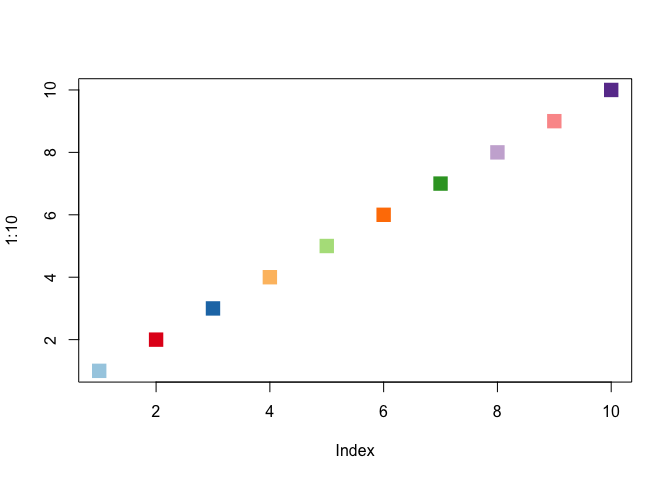
\includegraphics{vaccination-indicators_files/figure-latex/unnamed-chunk-4-1.pdf}

\begin{Shaded}
\begin{Highlighting}[]
\FunctionTok{source}\NormalTok{(}\StringTok{"2\_plot{-}overTime.R"}\NormalTok{)}
\end{Highlighting}
\end{Shaded}

\hypertarget{computation}{%
\section{Computation}\label{computation}}

\hypertarget{across-median-comparison}{%
\subsection{Across median comparison}\label{across-median-comparison}}

\begin{Shaded}
\begin{Highlighting}[]
\ControlFlowTok{if}\NormalTok{(runComputations)\{}
  \CommentTok{\# Define the combinations of parameters to be tested}
\NormalTok{  parmsLR }\OtherTok{\textless{}{-}} \FunctionTok{expand.grid}\NormalTok{(}\AttributeTok{varPred =} \FunctionTok{names}\NormalTok{(dat.nocorr)[}\SpecialCharTok{{-}}\DecValTok{1}\NormalTok{], }
                         \AttributeTok{thedate =} \FunctionTok{c}\NormalTok{(date1, date2, date3, date4), }
                         \AttributeTok{predTransform =} \StringTok{"discretize\_factor"}\NormalTok{, }
                         \AttributeTok{vaccAge =} \StringTok{"adults"}\NormalTok{, }
                         \AttributeTok{by.prbs =} \FloatTok{0.5}\NormalTok{, }
                         \AttributeTok{permutation =} \ConstantTok{FALSE}\NormalTok{,}
                         \AttributeTok{stringsAsFactors =} \ConstantTok{FALSE}\NormalTok{)}
  \CommentTok{\# Permutation }
  \CommentTok{\# Number of repetitions}
\NormalTok{  nrep }\OtherTok{\textless{}{-}} \DecValTok{1000}
  \CommentTok{\# Base combination of parameters}
\NormalTok{  tmpparmsPerm }\OtherTok{\textless{}{-}} \FunctionTok{expand.grid}\NormalTok{(}\AttributeTok{varPred =} \StringTok{"French\_nlty"}\NormalTok{, }
                              \AttributeTok{thedate =} \FunctionTok{c}\NormalTok{(date1, date2, date3, date4), }
                              \AttributeTok{predTransform =} \StringTok{"discretize\_factor"}\NormalTok{, }
                              \AttributeTok{vaccAge =} \StringTok{"adults"}\NormalTok{, }
                              \AttributeTok{by.prbs =} \FloatTok{0.5}\NormalTok{, }
                              \AttributeTok{permutation =} \ConstantTok{TRUE}\NormalTok{,}
                              \AttributeTok{stringsAsFactors =} \ConstantTok{FALSE}\NormalTok{)}
  \CommentTok{\# Add repeated parameters}
  \ControlFlowTok{for}\NormalTok{(i }\ControlFlowTok{in} \DecValTok{1}\SpecialCharTok{:}\NormalTok{nrep)\{}
\NormalTok{    parmsLR }\OtherTok{\textless{}{-}} \FunctionTok{rbind}\NormalTok{(parmsLR, tmpparmsPerm)}
\NormalTok{  \}}
  \FunctionTok{rm}\NormalTok{(tmpparmsPerm)}
  
  \CommentTok{\# Initialize output}
\NormalTok{  out }\OtherTok{\textless{}{-}} \FunctionTok{as.data.frame}\NormalTok{(}\FunctionTok{matrix}\NormalTok{(}\ConstantTok{NA}\NormalTok{, }\AttributeTok{ncol =} \DecValTok{8}\NormalTok{, }\AttributeTok{nrow =} \FunctionTok{nrow}\NormalTok{(parmsLR)))}
  \FunctionTok{cat}\NormalTok{(}\FunctionTok{nrow}\NormalTok{(parmsLR), }\StringTok{" combinations to be tested}\SpecialCharTok{\textbackslash{}n}\StringTok{"}\NormalTok{)}
  \CommentTok{\# Compute OR for each combination of parameters}
  \ControlFlowTok{for}\NormalTok{(i }\ControlFlowTok{in} \DecValTok{1}\SpecialCharTok{:}\FunctionTok{nrow}\NormalTok{(parmsLR))\{}
    \ControlFlowTok{if}\NormalTok{(i }\SpecialCharTok{\%\%} \DecValTok{10} \SpecialCharTok{==} \DecValTok{0}\NormalTok{) }\FunctionTok{cat}\NormalTok{(i, }\StringTok{""}\NormalTok{) }\CommentTok{\# Print counter}
    \CommentTok{\# Compute the logistic regression on this combination of parameters}
\NormalTok{    mdl }\OtherTok{\textless{}{-}} \FunctionTok{do.call}\NormalTok{(getLogReg, parmsLR[i, ])}
    \CommentTok{\# Extract the odds ratios}
\NormalTok{    out[i, ] }\OtherTok{\textless{}{-}} \FunctionTok{extractOR}\NormalTok{(mdl)}
\NormalTok{  \}}
  \FunctionTok{names}\NormalTok{(out) }\OtherTok{\textless{}{-}} \FunctionTok{names}\NormalTok{(}\FunctionTok{extractOR}\NormalTok{(mdl))}
  
  \CommentTok{\# Add the parameters}
\NormalTok{  outLR }\OtherTok{\textless{}{-}} \FunctionTok{cbind}\NormalTok{(parmsLR, out)}
  
  \CommentTok{\# Add type of predictor information}
\NormalTok{  outLR}\SpecialCharTok{$}\NormalTok{typePred }\OtherTok{\textless{}{-}}\NormalTok{ dicPred[outLR}\SpecialCharTok{$}\NormalTok{varPred]}
  \CommentTok{\# Full names}
\NormalTok{  outLR}\SpecialCharTok{$}\NormalTok{typePredFull }\OtherTok{\textless{}{-}}\NormalTok{ dic.fullpred[outLR}\SpecialCharTok{$}\NormalTok{typePred]}
  
  \FunctionTok{save}\NormalTok{(outLR, }\AttributeTok{file =} \StringTok{"outLR.RData"}\NormalTok{)}
  
\NormalTok{\}}
\end{Highlighting}
\end{Shaded}

\begin{Shaded}
\begin{Highlighting}[]
\FunctionTok{load}\NormalTok{(}\StringTok{"outLR.RData"}\NormalTok{)}

\CommentTok{\# PLOT}
\FunctionTok{plotManhattan}\NormalTok{(outLR, }\AttributeTok{ntop =} \DecValTok{5}\NormalTok{)}
\end{Highlighting}
\end{Shaded}

\begin{verbatim}
## Warning in text.default(y = tmp$i, x = tmp$OR.abs, adj = c(0, 0.5), labels =
## paste0(" ", : conversion failure on ' Unemployment_Benef ▼' in 'mbcsToSbcs':
## dot substituted for <e2>
\end{verbatim}

\begin{verbatim}
## Warning in text.default(y = tmp$i, x = tmp$OR.abs, adj = c(0, 0.5), labels =
## paste0(" ", : conversion failure on ' Unemployment_Benef ▼' in 'mbcsToSbcs':
## dot substituted for <96>
\end{verbatim}

\begin{verbatim}
## Warning in text.default(y = tmp$i, x = tmp$OR.abs, adj = c(0, 0.5), labels =
## paste0(" ", : conversion failure on ' Unemployment_Benef ▼' in 'mbcsToSbcs':
## dot substituted for <bc>
\end{verbatim}

\begin{verbatim}
## Warning in text.default(y = tmp$i, x = tmp$OR.abs, adj = c(0, 0.5), labels
## = paste0(" ", : conversion failure on ' Asselineau ▼' in 'mbcsToSbcs': dot
## substituted for <e2>
\end{verbatim}

\begin{verbatim}
## Warning in text.default(y = tmp$i, x = tmp$OR.abs, adj = c(0, 0.5), labels
## = paste0(" ", : conversion failure on ' Asselineau ▼' in 'mbcsToSbcs': dot
## substituted for <96>
\end{verbatim}

\begin{verbatim}
## Warning in text.default(y = tmp$i, x = tmp$OR.abs, adj = c(0, 0.5), labels
## = paste0(" ", : conversion failure on ' Asselineau ▼' in 'mbcsToSbcs': dot
## substituted for <bc>
\end{verbatim}

\begin{verbatim}
## Warning in text.default(y = tmp$i, x = tmp$OR.abs, adj = c(0, 0.5), labels
## = paste0(" ", : conversion failure on ' 2554_women_Workforce_rate ▲' in
## 'mbcsToSbcs': dot substituted for <e2>
\end{verbatim}

\begin{verbatim}
## Warning in text.default(y = tmp$i, x = tmp$OR.abs, adj = c(0, 0.5), labels
## = paste0(" ", : conversion failure on ' 2554_women_Workforce_rate ▲' in
## 'mbcsToSbcs': dot substituted for <96>
\end{verbatim}

\begin{verbatim}
## Warning in text.default(y = tmp$i, x = tmp$OR.abs, adj = c(0, 0.5), labels
## = paste0(" ", : conversion failure on ' 2554_women_Workforce_rate ▲' in
## 'mbcsToSbcs': dot substituted for <b2>
\end{verbatim}

\begin{verbatim}
## Warning in text.default(y = tmp$i, x = tmp$OR.abs, adj = c(0, 0.5), labels
## = paste0(" ", : conversion failure on ' Abstention ▼' in 'mbcsToSbcs': dot
## substituted for <e2>
\end{verbatim}

\begin{verbatim}
## Warning in text.default(y = tmp$i, x = tmp$OR.abs, adj = c(0, 0.5), labels
## = paste0(" ", : conversion failure on ' Abstention ▼' in 'mbcsToSbcs': dot
## substituted for <96>
\end{verbatim}

\begin{verbatim}
## Warning in text.default(y = tmp$i, x = tmp$OR.abs, adj = c(0, 0.5), labels
## = paste0(" ", : conversion failure on ' Abstention ▼' in 'mbcsToSbcs': dot
## substituted for <bc>
\end{verbatim}

\begin{verbatim}
## Warning in text.default(y = tmp$i, x = tmp$OR.abs, adj = c(0, 0.5), labels =
## paste0(" ", : conversion failure on ' D1_st_Living ▲' in 'mbcsToSbcs': dot
## substituted for <e2>
\end{verbatim}

\begin{verbatim}
## Warning in text.default(y = tmp$i, x = tmp$OR.abs, adj = c(0, 0.5), labels =
## paste0(" ", : conversion failure on ' D1_st_Living ▲' in 'mbcsToSbcs': dot
## substituted for <96>
\end{verbatim}

\begin{verbatim}
## Warning in text.default(y = tmp$i, x = tmp$OR.abs, adj = c(0, 0.5), labels =
## paste0(" ", : conversion failure on ' D1_st_Living ▲' in 'mbcsToSbcs': dot
## substituted for <b2>
\end{verbatim}

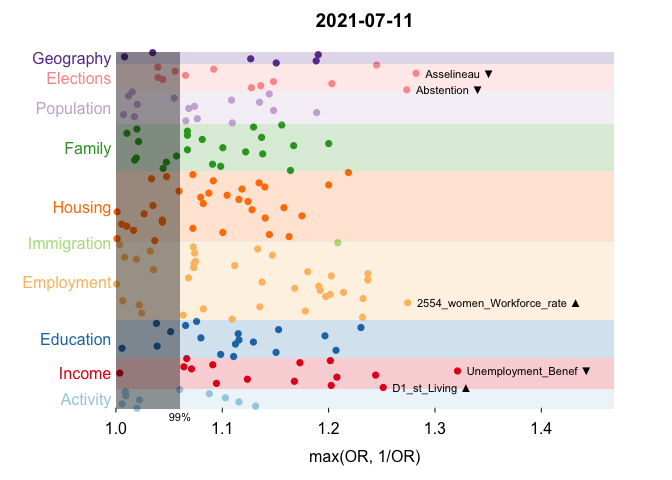
\includegraphics{vaccination-indicators_files/figure-latex/manhattan_median-1.pdf}

\begin{verbatim}
## Warning in text.default(y = tmp$i, x = tmp$OR.abs, adj = c(0, 0.5), labels =
## paste0(" ", : conversion failure on ' Unemployment_Benef ▼' in 'mbcsToSbcs':
## dot substituted for <e2>
\end{verbatim}

\begin{verbatim}
## Warning in text.default(y = tmp$i, x = tmp$OR.abs, adj = c(0, 0.5), labels =
## paste0(" ", : conversion failure on ' Unemployment_Benef ▼' in 'mbcsToSbcs':
## dot substituted for <96>
\end{verbatim}

\begin{verbatim}
## Warning in text.default(y = tmp$i, x = tmp$OR.abs, adj = c(0, 0.5), labels =
## paste0(" ", : conversion failure on ' Unemployment_Benef ▼' in 'mbcsToSbcs':
## dot substituted for <bc>
\end{verbatim}

\begin{verbatim}
## Warning in text.default(y = tmp$i, x = tmp$OR.abs, adj = c(0, 0.5), labels
## = paste0(" ", : conversion failure on ' Asselineau ▼' in 'mbcsToSbcs': dot
## substituted for <e2>
\end{verbatim}

\begin{verbatim}
## Warning in text.default(y = tmp$i, x = tmp$OR.abs, adj = c(0, 0.5), labels
## = paste0(" ", : conversion failure on ' Asselineau ▼' in 'mbcsToSbcs': dot
## substituted for <96>
\end{verbatim}

\begin{verbatim}
## Warning in text.default(y = tmp$i, x = tmp$OR.abs, adj = c(0, 0.5), labels
## = paste0(" ", : conversion failure on ' Asselineau ▼' in 'mbcsToSbcs': dot
## substituted for <bc>
\end{verbatim}

\begin{verbatim}
## Warning in text.default(y = tmp$i, x = tmp$OR.abs, adj = c(0, 0.5), labels
## = paste0(" ", : conversion failure on ' 2554_women_Workforce_rate ▲' in
## 'mbcsToSbcs': dot substituted for <e2>
\end{verbatim}

\begin{verbatim}
## Warning in text.default(y = tmp$i, x = tmp$OR.abs, adj = c(0, 0.5), labels
## = paste0(" ", : conversion failure on ' 2554_women_Workforce_rate ▲' in
## 'mbcsToSbcs': dot substituted for <96>
\end{verbatim}

\begin{verbatim}
## Warning in text.default(y = tmp$i, x = tmp$OR.abs, adj = c(0, 0.5), labels
## = paste0(" ", : conversion failure on ' 2554_women_Workforce_rate ▲' in
## 'mbcsToSbcs': dot substituted for <b2>
\end{verbatim}

\begin{verbatim}
## Warning in text.default(y = tmp$i, x = tmp$OR.abs, adj = c(0, 0.5), labels
## = paste0(" ", : conversion failure on ' Abstention ▼' in 'mbcsToSbcs': dot
## substituted for <e2>
\end{verbatim}

\begin{verbatim}
## Warning in text.default(y = tmp$i, x = tmp$OR.abs, adj = c(0, 0.5), labels
## = paste0(" ", : conversion failure on ' Abstention ▼' in 'mbcsToSbcs': dot
## substituted for <96>
\end{verbatim}

\begin{verbatim}
## Warning in text.default(y = tmp$i, x = tmp$OR.abs, adj = c(0, 0.5), labels
## = paste0(" ", : conversion failure on ' Abstention ▼' in 'mbcsToSbcs': dot
## substituted for <bc>
\end{verbatim}

\begin{verbatim}
## Warning in text.default(y = tmp$i, x = tmp$OR.abs, adj = c(0, 0.5), labels =
## paste0(" ", : conversion failure on ' D1_st_Living ▲' in 'mbcsToSbcs': dot
## substituted for <e2>
\end{verbatim}

\begin{verbatim}
## Warning in text.default(y = tmp$i, x = tmp$OR.abs, adj = c(0, 0.5), labels =
## paste0(" ", : conversion failure on ' D1_st_Living ▲' in 'mbcsToSbcs': dot
## substituted for <96>
\end{verbatim}

\begin{verbatim}
## Warning in text.default(y = tmp$i, x = tmp$OR.abs, adj = c(0, 0.5), labels =
## paste0(" ", : conversion failure on ' D1_st_Living ▲' in 'mbcsToSbcs': dot
## substituted for <b2>
\end{verbatim}

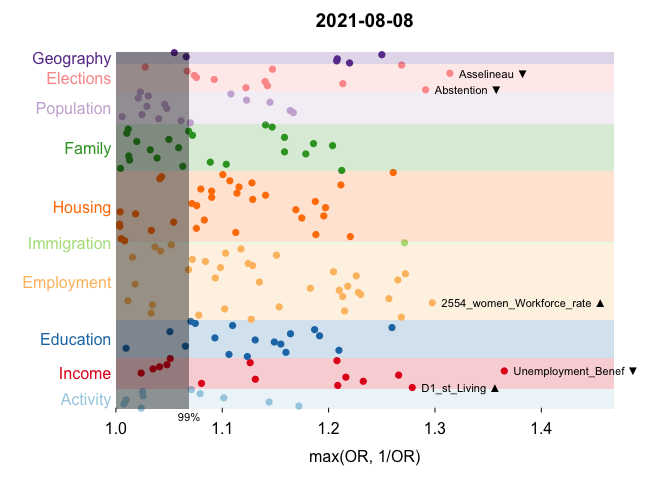
\includegraphics{vaccination-indicators_files/figure-latex/manhattan_median-2.pdf}

\begin{verbatim}
## Warning in text.default(y = tmp$i, x = tmp$OR.abs, adj = c(0, 0.5), labels =
## paste0(" ", : conversion failure on ' Unemployment_Benef ▼' in 'mbcsToSbcs':
## dot substituted for <e2>
\end{verbatim}

\begin{verbatim}
## Warning in text.default(y = tmp$i, x = tmp$OR.abs, adj = c(0, 0.5), labels =
## paste0(" ", : conversion failure on ' Unemployment_Benef ▼' in 'mbcsToSbcs':
## dot substituted for <96>
\end{verbatim}

\begin{verbatim}
## Warning in text.default(y = tmp$i, x = tmp$OR.abs, adj = c(0, 0.5), labels =
## paste0(" ", : conversion failure on ' Unemployment_Benef ▼' in 'mbcsToSbcs':
## dot substituted for <bc>
\end{verbatim}

\begin{verbatim}
## Warning in text.default(y = tmp$i, x = tmp$OR.abs, adj = c(0, 0.5), labels
## = paste0(" ", : conversion failure on ' Asselineau ▼' in 'mbcsToSbcs': dot
## substituted for <e2>
\end{verbatim}

\begin{verbatim}
## Warning in text.default(y = tmp$i, x = tmp$OR.abs, adj = c(0, 0.5), labels
## = paste0(" ", : conversion failure on ' Asselineau ▼' in 'mbcsToSbcs': dot
## substituted for <96>
\end{verbatim}

\begin{verbatim}
## Warning in text.default(y = tmp$i, x = tmp$OR.abs, adj = c(0, 0.5), labels
## = paste0(" ", : conversion failure on ' Asselineau ▼' in 'mbcsToSbcs': dot
## substituted for <bc>
\end{verbatim}

\begin{verbatim}
## Warning in text.default(y = tmp$i, x = tmp$OR.abs, adj = c(0, 0.5), labels
## = paste0(" ", : conversion failure on ' Immigrant ▼' in 'mbcsToSbcs': dot
## substituted for <e2>
\end{verbatim}

\begin{verbatim}
## Warning in text.default(y = tmp$i, x = tmp$OR.abs, adj = c(0, 0.5), labels
## = paste0(" ", : conversion failure on ' Immigrant ▼' in 'mbcsToSbcs': dot
## substituted for <96>
\end{verbatim}

\begin{verbatim}
## Warning in text.default(y = tmp$i, x = tmp$OR.abs, adj = c(0, 0.5), labels
## = paste0(" ", : conversion failure on ' Immigrant ▼' in 'mbcsToSbcs': dot
## substituted for <bc>
\end{verbatim}

\begin{verbatim}
## Warning in text.default(y = tmp$i, x = tmp$OR.abs, adj = c(0, 0.5), labels =
## paste0(" ", : conversion failure on ' Overcrowding_rate ▼' in 'mbcsToSbcs': dot
## substituted for <e2>
\end{verbatim}

\begin{verbatim}
## Warning in text.default(y = tmp$i, x = tmp$OR.abs, adj = c(0, 0.5), labels =
## paste0(" ", : conversion failure on ' Overcrowding_rate ▼' in 'mbcsToSbcs': dot
## substituted for <96>
\end{verbatim}

\begin{verbatim}
## Warning in text.default(y = tmp$i, x = tmp$OR.abs, adj = c(0, 0.5), labels =
## paste0(" ", : conversion failure on ' Overcrowding_rate ▼' in 'mbcsToSbcs': dot
## substituted for <bc>
\end{verbatim}

\begin{verbatim}
## Warning in text.default(y = tmp$i, x = tmp$OR.abs, adj = c(0, 0.5), labels
## = paste0(" ", : conversion failure on ' 2554_women_Workforce_rate ▲' in
## 'mbcsToSbcs': dot substituted for <e2>
\end{verbatim}

\begin{verbatim}
## Warning in text.default(y = tmp$i, x = tmp$OR.abs, adj = c(0, 0.5), labels
## = paste0(" ", : conversion failure on ' 2554_women_Workforce_rate ▲' in
## 'mbcsToSbcs': dot substituted for <96>
\end{verbatim}

\begin{verbatim}
## Warning in text.default(y = tmp$i, x = tmp$OR.abs, adj = c(0, 0.5), labels
## = paste0(" ", : conversion failure on ' 2554_women_Workforce_rate ▲' in
## 'mbcsToSbcs': dot substituted for <b2>
\end{verbatim}

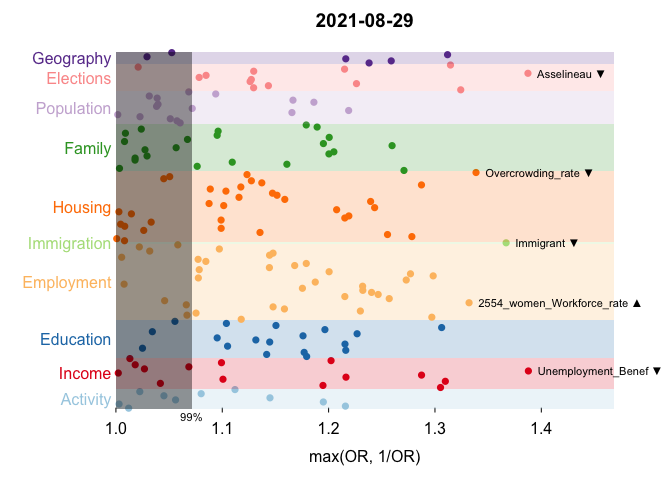
\includegraphics{vaccination-indicators_files/figure-latex/manhattan_median-3.pdf}

\begin{verbatim}
## Warning in text.default(y = tmp$i, x = tmp$OR.abs, adj = c(0, 0.5), labels =
## paste0(" ", : conversion failure on ' Unemployment_Benef ▼' in 'mbcsToSbcs':
## dot substituted for <e2>
\end{verbatim}

\begin{verbatim}
## Warning in text.default(y = tmp$i, x = tmp$OR.abs, adj = c(0, 0.5), labels =
## paste0(" ", : conversion failure on ' Unemployment_Benef ▼' in 'mbcsToSbcs':
## dot substituted for <96>
\end{verbatim}

\begin{verbatim}
## Warning in text.default(y = tmp$i, x = tmp$OR.abs, adj = c(0, 0.5), labels =
## paste0(" ", : conversion failure on ' Unemployment_Benef ▼' in 'mbcsToSbcs':
## dot substituted for <bc>
\end{verbatim}

\begin{verbatim}
## Warning in text.default(y = tmp$i, x = tmp$OR.abs, adj = c(0, 0.5), labels
## = paste0(" ", : conversion failure on ' Asselineau ▼' in 'mbcsToSbcs': dot
## substituted for <e2>
\end{verbatim}

\begin{verbatim}
## Warning in text.default(y = tmp$i, x = tmp$OR.abs, adj = c(0, 0.5), labels
## = paste0(" ", : conversion failure on ' Asselineau ▼' in 'mbcsToSbcs': dot
## substituted for <96>
\end{verbatim}

\begin{verbatim}
## Warning in text.default(y = tmp$i, x = tmp$OR.abs, adj = c(0, 0.5), labels
## = paste0(" ", : conversion failure on ' Asselineau ▼' in 'mbcsToSbcs': dot
## substituted for <bc>
\end{verbatim}

\begin{verbatim}
## Warning in text.default(y = tmp$i, x = tmp$OR.abs, adj = c(0, 0.5), labels
## = paste0(" ", : conversion failure on ' Immigrant ▼' in 'mbcsToSbcs': dot
## substituted for <e2>
\end{verbatim}

\begin{verbatim}
## Warning in text.default(y = tmp$i, x = tmp$OR.abs, adj = c(0, 0.5), labels
## = paste0(" ", : conversion failure on ' Immigrant ▼' in 'mbcsToSbcs': dot
## substituted for <96>
\end{verbatim}

\begin{verbatim}
## Warning in text.default(y = tmp$i, x = tmp$OR.abs, adj = c(0, 0.5), labels
## = paste0(" ", : conversion failure on ' Immigrant ▼' in 'mbcsToSbcs': dot
## substituted for <bc>
\end{verbatim}

\begin{verbatim}
## Warning in text.default(y = tmp$i, x = tmp$OR.abs, adj = c(0, 0.5), labels =
## paste0(" ", : conversion failure on ' Overcrowding_rate ▼' in 'mbcsToSbcs': dot
## substituted for <e2>
\end{verbatim}

\begin{verbatim}
## Warning in text.default(y = tmp$i, x = tmp$OR.abs, adj = c(0, 0.5), labels =
## paste0(" ", : conversion failure on ' Overcrowding_rate ▼' in 'mbcsToSbcs': dot
## substituted for <96>
\end{verbatim}

\begin{verbatim}
## Warning in text.default(y = tmp$i, x = tmp$OR.abs, adj = c(0, 0.5), labels =
## paste0(" ", : conversion failure on ' Overcrowding_rate ▼' in 'mbcsToSbcs': dot
## substituted for <bc>
\end{verbatim}

\begin{verbatim}
## Warning in text.default(y = tmp$i, x = tmp$OR.abs, adj = c(0, 0.5), labels =
## paste0(" ", : conversion failure on ' NO.SE ▼' in 'mbcsToSbcs': dot substituted
## for <e2>
\end{verbatim}

\begin{verbatim}
## Warning in text.default(y = tmp$i, x = tmp$OR.abs, adj = c(0, 0.5), labels =
## paste0(" ", : conversion failure on ' NO.SE ▼' in 'mbcsToSbcs': dot substituted
## for <96>
\end{verbatim}

\begin{verbatim}
## Warning in text.default(y = tmp$i, x = tmp$OR.abs, adj = c(0, 0.5), labels =
## paste0(" ", : conversion failure on ' NO.SE ▼' in 'mbcsToSbcs': dot substituted
## for <bc>
\end{verbatim}

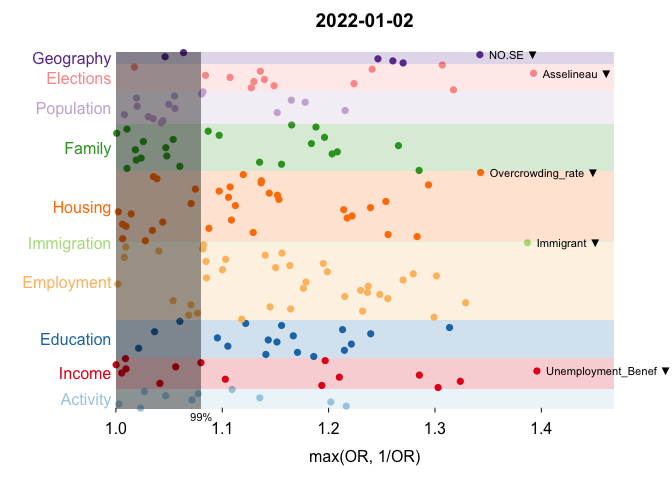
\includegraphics{vaccination-indicators_files/figure-latex/manhattan_median-4.pdf}

\hypertarget{by-deciles-quantitatively-adjusting-ages}{%
\subsection{By deciles, quantitatively, adjusting
ages}\label{by-deciles-quantitatively-adjusting-ages}}

\begin{Shaded}
\begin{Highlighting}[]
\ControlFlowTok{if}\NormalTok{(runComputations)\{}
  \CommentTok{\# Define the combinations of parameters to be tested}
\NormalTok{  parmsDec }\OtherTok{\textless{}{-}} \FunctionTok{expand.grid}\NormalTok{(}\AttributeTok{varPred =} \FunctionTok{names}\NormalTok{(dat.nocorr)[}\SpecialCharTok{{-}}\DecValTok{1}\NormalTok{], }
                          \AttributeTok{thedate =} \FunctionTok{c}\NormalTok{(date1, date2, date3, date4), }
                          \AttributeTok{predTransform =} \StringTok{"discretize"}\NormalTok{, }
                          \AttributeTok{vaccAge =} \StringTok{"by\_age"}\NormalTok{, }
                          \AttributeTok{by.prbs =} \FloatTok{0.1}\NormalTok{, }
                          \AttributeTok{permutation =} \ConstantTok{FALSE}\NormalTok{,}
                          \AttributeTok{stringsAsFactors =} \ConstantTok{FALSE}\NormalTok{)}
  
  \CommentTok{\# Permutation}
  \CommentTok{\# Base combination of parameters}
\NormalTok{  tmpparmsPerm }\OtherTok{\textless{}{-}} \FunctionTok{expand.grid}\NormalTok{(}\AttributeTok{varPred =} \StringTok{"French\_nlty"}\NormalTok{, }
                              \AttributeTok{thedate =} \FunctionTok{c}\NormalTok{(date1, date2, date3, date4), }
                              \AttributeTok{predTransform =} \StringTok{"discretize"}\NormalTok{, }
                              \AttributeTok{vaccAge =} \StringTok{"by\_age"}\NormalTok{, }
                              \AttributeTok{by.prbs =} \FloatTok{0.1}\NormalTok{, }
                              \AttributeTok{permutation =} \ConstantTok{TRUE}\NormalTok{,}
                              \AttributeTok{stringsAsFactors =} \ConstantTok{FALSE}\NormalTok{)}
  \CommentTok{\# Add repeated parameters}
  \ControlFlowTok{for}\NormalTok{(i }\ControlFlowTok{in} \DecValTok{1}\SpecialCharTok{:}\NormalTok{nrep)\{}
\NormalTok{    parmsDec }\OtherTok{\textless{}{-}} \FunctionTok{rbind}\NormalTok{(parmsDec, tmpparmsPerm)}
\NormalTok{  \}}
  \FunctionTok{rm}\NormalTok{(tmpparmsPerm)}
  
  
\NormalTok{  newd }\OtherTok{\textless{}{-}} \FunctionTok{expand.grid}\NormalTok{(}\AttributeTok{age.f =} \FunctionTok{as.factor}\NormalTok{(ages), }\AttributeTok{pred.std =} \DecValTok{1}\SpecialCharTok{:}\DecValTok{10}\NormalTok{)}
  
  
  \FunctionTok{cat}\NormalTok{(}\FunctionTok{nrow}\NormalTok{(parmsDec), }\StringTok{" combinations to be tested}\SpecialCharTok{\textbackslash{}n}\StringTok{"}\NormalTok{)}
  
  
\NormalTok{  out }\OtherTok{\textless{}{-}} \FunctionTok{as.data.frame}\NormalTok{(}\FunctionTok{matrix}\NormalTok{(}\ConstantTok{NA}\NormalTok{, }\AttributeTok{ncol =} \DecValTok{4}\NormalTok{, }\AttributeTok{nrow =} \FunctionTok{nrow}\NormalTok{(parmsDec)))}
  
  \CommentTok{\# Compute OR for each combination of parameters}
  \ControlFlowTok{for}\NormalTok{(i }\ControlFlowTok{in} \DecValTok{1}\SpecialCharTok{:}\FunctionTok{nrow}\NormalTok{(parmsDec))\{}
    \ControlFlowTok{if}\NormalTok{(i }\SpecialCharTok{\%\%} \DecValTok{10} \SpecialCharTok{==} \DecValTok{0}\NormalTok{) }\FunctionTok{cat}\NormalTok{(i, }\StringTok{""}\NormalTok{) }\CommentTok{\# Print counter}
    \CommentTok{\# Compute the logistic regression on this combination of parameters}
\NormalTok{    mdl }\OtherTok{\textless{}{-}} \FunctionTok{do.call}\NormalTok{(getLogReg, parmsDec[i, ])}
    \CommentTok{\# Predicted values}
\NormalTok{    predsC }\OtherTok{\textless{}{-}} \FunctionTok{adjustedPredict}\NormalTok{(mdl, newd, }\AttributeTok{includeChildren =} \ConstantTok{TRUE}\NormalTok{)}
\NormalTok{    predsA }\OtherTok{\textless{}{-}} \FunctionTok{adjustedPredict}\NormalTok{(mdl, newd, }\AttributeTok{includeChildren =} \ConstantTok{FALSE}\NormalTok{)}
    
    \CommentTok{\# Compute odds ratios}
\NormalTok{    ORC }\OtherTok{\textless{}{-}} \FunctionTok{getORfromPredict}\NormalTok{(}\FunctionTok{c}\NormalTok{(predsC[predsC}\SpecialCharTok{$}\NormalTok{pred.std }\SpecialCharTok{==} \DecValTok{10}\NormalTok{, }\StringTok{"adjustedRate"}\NormalTok{], predsC[predsC}\SpecialCharTok{$}\NormalTok{pred.std }\SpecialCharTok{==} \DecValTok{1}\NormalTok{, }\StringTok{"adjustedRate"}\NormalTok{]))}
\NormalTok{    ORA }\OtherTok{\textless{}{-}} \FunctionTok{getORfromPredict}\NormalTok{(}\FunctionTok{c}\NormalTok{(predsA[predsA}\SpecialCharTok{$}\NormalTok{pred.std }\SpecialCharTok{==} \DecValTok{10}\NormalTok{, }\StringTok{"adjustedRate"}\NormalTok{], predsA[predsA}\SpecialCharTok{$}\NormalTok{pred.std }\SpecialCharTok{==} \DecValTok{1}\NormalTok{, }\StringTok{"adjustedRate"}\NormalTok{]))}
    
\NormalTok{    out[i, ] }\OtherTok{\textless{}{-}} \FunctionTok{c}\NormalTok{(ORC, ORA, }\FunctionTok{max}\NormalTok{(ORC, }\DecValTok{1}\SpecialCharTok{/}\NormalTok{ORC), }\FunctionTok{max}\NormalTok{(ORA, }\DecValTok{1}\SpecialCharTok{/}\NormalTok{ORA))}
\NormalTok{  \}}
  \FunctionTok{names}\NormalTok{(out) }\OtherTok{\textless{}{-}} \FunctionTok{c}\NormalTok{(}\StringTok{"OR.withChildren"}\NormalTok{, }\StringTok{"OR.adults"}\NormalTok{, }\StringTok{"OR.abs.withChildren"}\NormalTok{, }\StringTok{"OR.abs.adults"}\NormalTok{)}
  \FunctionTok{dim}\NormalTok{(out)}
  \CommentTok{\# Add the parameters}
\NormalTok{  outDec }\OtherTok{\textless{}{-}} \FunctionTok{cbind}\NormalTok{(parmsDec, out)}
  \CommentTok{\# Add type of predictor information}
\NormalTok{  outDec}\SpecialCharTok{$}\NormalTok{typePred }\OtherTok{\textless{}{-}}\NormalTok{ dicPred[outDec}\SpecialCharTok{$}\NormalTok{varPred]}
  \CommentTok{\# Full names}
\NormalTok{  outDec}\SpecialCharTok{$}\NormalTok{typePredFull }\OtherTok{\textless{}{-}}\NormalTok{ dic.fullpred[outDec}\SpecialCharTok{$}\NormalTok{typePred]}
  
  \FunctionTok{save}\NormalTok{(outDec, }\AttributeTok{file =} \StringTok{"outDec.RData"}\NormalTok{)}
  
\NormalTok{\}}
\end{Highlighting}
\end{Shaded}

\begin{Shaded}
\begin{Highlighting}[]
\FunctionTok{load}\NormalTok{(}\StringTok{"outDec.RData"}\NormalTok{)}

\NormalTok{suffix }\OtherTok{\textless{}{-}} \StringTok{".withChildren"}

\NormalTok{xx }\OtherTok{\textless{}{-}}\NormalTok{ outDec}
\NormalTok{xx}\SpecialCharTok{$}\NormalTok{OR }\OtherTok{\textless{}{-}}\NormalTok{ outDec[, }\FunctionTok{paste0}\NormalTok{(}\StringTok{"OR"}\NormalTok{, suffix)]}
\NormalTok{xx}\SpecialCharTok{$}\NormalTok{OR.abs }\OtherTok{\textless{}{-}}\NormalTok{ outDec[, }\FunctionTok{paste0}\NormalTok{(}\StringTok{"OR.abs"}\NormalTok{, suffix)]}
\NormalTok{xx}\SpecialCharTok{$}\NormalTok{OR.abs.CI.max }\OtherTok{\textless{}{-}}\NormalTok{ outDec[, }\FunctionTok{paste0}\NormalTok{(}\StringTok{"OR.abs"}\NormalTok{, suffix)]}

\FunctionTok{plotManhattan}\NormalTok{(xx, }\AttributeTok{ntop =} \DecValTok{5}\NormalTok{)}
\end{Highlighting}
\end{Shaded}

\begin{verbatim}
## Warning in text.default(y = tmp$i, x = tmp$OR.abs, adj = c(0, 0.5), labels
## = paste0(" ", : conversion failure on ' 1564_OtherInactive_amg_NW ▼' in
## 'mbcsToSbcs': dot substituted for <e2>
\end{verbatim}

\begin{verbatim}
## Warning in text.default(y = tmp$i, x = tmp$OR.abs, adj = c(0, 0.5), labels
## = paste0(" ", : conversion failure on ' 1564_OtherInactive_amg_NW ▼' in
## 'mbcsToSbcs': dot substituted for <96>
\end{verbatim}

\begin{verbatim}
## Warning in text.default(y = tmp$i, x = tmp$OR.abs, adj = c(0, 0.5), labels
## = paste0(" ", : conversion failure on ' 1564_OtherInactive_amg_NW ▼' in
## 'mbcsToSbcs': dot substituted for <bc>
\end{verbatim}

\begin{verbatim}
## Warning in text.default(y = tmp$i, x = tmp$OR.abs, adj = c(0, 0.5), labels
## = paste0(" ", : conversion failure on ' 1564_OtherInactive_amg_WF ▼' in
## 'mbcsToSbcs': dot substituted for <e2>
\end{verbatim}

\begin{verbatim}
## Warning in text.default(y = tmp$i, x = tmp$OR.abs, adj = c(0, 0.5), labels
## = paste0(" ", : conversion failure on ' 1564_OtherInactive_amg_WF ▼' in
## 'mbcsToSbcs': dot substituted for <96>
\end{verbatim}

\begin{verbatim}
## Warning in text.default(y = tmp$i, x = tmp$OR.abs, adj = c(0, 0.5), labels
## = paste0(" ", : conversion failure on ' 1564_OtherInactive_amg_WF ▼' in
## 'mbcsToSbcs': dot substituted for <bc>
\end{verbatim}

\begin{verbatim}
## Warning in text.default(y = tmp$i, x = tmp$OR.abs, adj = c(0, 0.5), labels =
## paste0(" ", : conversion failure on ' Unemployment_Benef ▼' in 'mbcsToSbcs':
## dot substituted for <e2>
\end{verbatim}

\begin{verbatim}
## Warning in text.default(y = tmp$i, x = tmp$OR.abs, adj = c(0, 0.5), labels =
## paste0(" ", : conversion failure on ' Unemployment_Benef ▼' in 'mbcsToSbcs':
## dot substituted for <96>
\end{verbatim}

\begin{verbatim}
## Warning in text.default(y = tmp$i, x = tmp$OR.abs, adj = c(0, 0.5), labels =
## paste0(" ", : conversion failure on ' Unemployment_Benef ▼' in 'mbcsToSbcs':
## dot substituted for <bc>
\end{verbatim}

\begin{verbatim}
## Warning in text.default(y = tmp$i, x = tmp$OR.abs, adj = c(0, 0.5), labels
## = paste0(" ", : conversion failure on ' 15._men_NoDiploma_amg_mWF ▼' in
## 'mbcsToSbcs': dot substituted for <e2>
\end{verbatim}

\begin{verbatim}
## Warning in text.default(y = tmp$i, x = tmp$OR.abs, adj = c(0, 0.5), labels
## = paste0(" ", : conversion failure on ' 15._men_NoDiploma_amg_mWF ▼' in
## 'mbcsToSbcs': dot substituted for <96>
\end{verbatim}

\begin{verbatim}
## Warning in text.default(y = tmp$i, x = tmp$OR.abs, adj = c(0, 0.5), labels
## = paste0(" ", : conversion failure on ' 15._men_NoDiploma_amg_mWF ▼' in
## 'mbcsToSbcs': dot substituted for <bc>
\end{verbatim}

\begin{verbatim}
## Warning in text.default(y = tmp$i, x = tmp$OR.abs, adj = c(0, 0.5), labels =
## paste0(" ", : conversion failure on ' Median_st_Living ▲' in 'mbcsToSbcs': dot
## substituted for <e2>
\end{verbatim}

\begin{verbatim}
## Warning in text.default(y = tmp$i, x = tmp$OR.abs, adj = c(0, 0.5), labels =
## paste0(" ", : conversion failure on ' Median_st_Living ▲' in 'mbcsToSbcs': dot
## substituted for <96>
\end{verbatim}

\begin{verbatim}
## Warning in text.default(y = tmp$i, x = tmp$OR.abs, adj = c(0, 0.5), labels =
## paste0(" ", : conversion failure on ' Median_st_Living ▲' in 'mbcsToSbcs': dot
## substituted for <b2>
\end{verbatim}

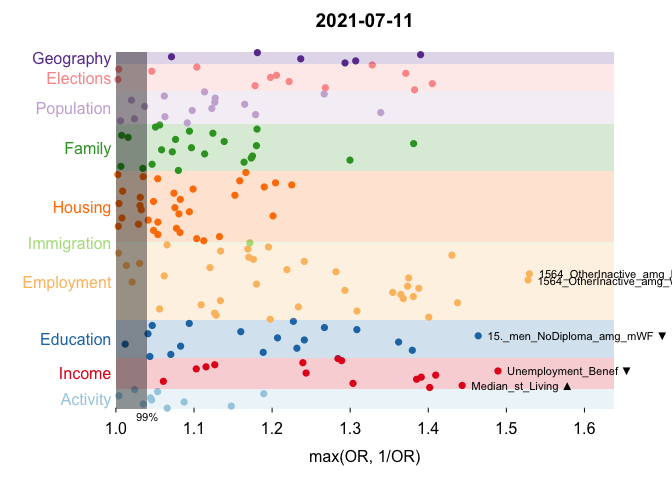
\includegraphics{vaccination-indicators_files/figure-latex/manhattan_decilesQ_withChildren-1.pdf}

\begin{verbatim}
## Warning in text.default(y = tmp$i, x = tmp$OR.abs, adj = c(0, 0.5), labels =
## paste0(" ", : conversion failure on ' Unemployment_Benef ▼' in 'mbcsToSbcs':
## dot substituted for <e2>
\end{verbatim}

\begin{verbatim}
## Warning in text.default(y = tmp$i, x = tmp$OR.abs, adj = c(0, 0.5), labels =
## paste0(" ", : conversion failure on ' Unemployment_Benef ▼' in 'mbcsToSbcs':
## dot substituted for <96>
\end{verbatim}

\begin{verbatim}
## Warning in text.default(y = tmp$i, x = tmp$OR.abs, adj = c(0, 0.5), labels =
## paste0(" ", : conversion failure on ' Unemployment_Benef ▼' in 'mbcsToSbcs':
## dot substituted for <bc>
\end{verbatim}

\begin{verbatim}
## Warning in text.default(y = tmp$i, x = tmp$OR.abs, adj = c(0, 0.5), labels
## = paste0(" ", : conversion failure on ' 1564_OtherInactive_amg_NW ▼' in
## 'mbcsToSbcs': dot substituted for <e2>
\end{verbatim}

\begin{verbatim}
## Warning in text.default(y = tmp$i, x = tmp$OR.abs, adj = c(0, 0.5), labels
## = paste0(" ", : conversion failure on ' 1564_OtherInactive_amg_NW ▼' in
## 'mbcsToSbcs': dot substituted for <96>
\end{verbatim}

\begin{verbatim}
## Warning in text.default(y = tmp$i, x = tmp$OR.abs, adj = c(0, 0.5), labels
## = paste0(" ", : conversion failure on ' 1564_OtherInactive_amg_NW ▼' in
## 'mbcsToSbcs': dot substituted for <bc>
\end{verbatim}

\begin{verbatim}
## Warning in text.default(y = tmp$i, x = tmp$OR.abs, adj = c(0, 0.5), labels
## = paste0(" ", : conversion failure on ' 1564_OtherInactive_amg_WF ▼' in
## 'mbcsToSbcs': dot substituted for <e2>
\end{verbatim}

\begin{verbatim}
## Warning in text.default(y = tmp$i, x = tmp$OR.abs, adj = c(0, 0.5), labels
## = paste0(" ", : conversion failure on ' 1564_OtherInactive_amg_WF ▼' in
## 'mbcsToSbcs': dot substituted for <96>
\end{verbatim}

\begin{verbatim}
## Warning in text.default(y = tmp$i, x = tmp$OR.abs, adj = c(0, 0.5), labels
## = paste0(" ", : conversion failure on ' 1564_OtherInactive_amg_WF ▼' in
## 'mbcsToSbcs': dot substituted for <bc>
\end{verbatim}

\begin{verbatim}
## Warning in text.default(y = tmp$i, x = tmp$OR.abs, adj = c(0, 0.5), labels
## = paste0(" ", : conversion failure on ' 2554_women_Workforce_rate ▲' in
## 'mbcsToSbcs': dot substituted for <e2>
\end{verbatim}

\begin{verbatim}
## Warning in text.default(y = tmp$i, x = tmp$OR.abs, adj = c(0, 0.5), labels
## = paste0(" ", : conversion failure on ' 2554_women_Workforce_rate ▲' in
## 'mbcsToSbcs': dot substituted for <96>
\end{verbatim}

\begin{verbatim}
## Warning in text.default(y = tmp$i, x = tmp$OR.abs, adj = c(0, 0.5), labels
## = paste0(" ", : conversion failure on ' 2554_women_Workforce_rate ▲' in
## 'mbcsToSbcs': dot substituted for <b2>
\end{verbatim}

\begin{verbatim}
## Warning in text.default(y = tmp$i, x = tmp$OR.abs, adj = c(0, 0.5), labels
## = paste0(" ", : conversion failure on ' Asselineau ▼' in 'mbcsToSbcs': dot
## substituted for <e2>
\end{verbatim}

\begin{verbatim}
## Warning in text.default(y = tmp$i, x = tmp$OR.abs, adj = c(0, 0.5), labels
## = paste0(" ", : conversion failure on ' Asselineau ▼' in 'mbcsToSbcs': dot
## substituted for <96>
\end{verbatim}

\begin{verbatim}
## Warning in text.default(y = tmp$i, x = tmp$OR.abs, adj = c(0, 0.5), labels
## = paste0(" ", : conversion failure on ' Asselineau ▼' in 'mbcsToSbcs': dot
## substituted for <bc>
\end{verbatim}

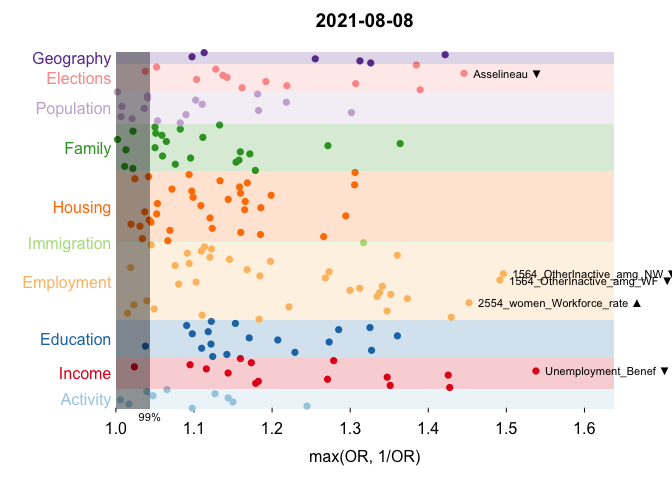
\includegraphics{vaccination-indicators_files/figure-latex/manhattan_decilesQ_withChildren-2.pdf}

\begin{verbatim}
## Warning in text.default(y = tmp$i, x = tmp$OR.abs, adj = c(0, 0.5), labels =
## paste0(" ", : conversion failure on ' Unemployment_Benef ▼' in 'mbcsToSbcs':
## dot substituted for <e2>
\end{verbatim}

\begin{verbatim}
## Warning in text.default(y = tmp$i, x = tmp$OR.abs, adj = c(0, 0.5), labels =
## paste0(" ", : conversion failure on ' Unemployment_Benef ▼' in 'mbcsToSbcs':
## dot substituted for <96>
\end{verbatim}

\begin{verbatim}
## Warning in text.default(y = tmp$i, x = tmp$OR.abs, adj = c(0, 0.5), labels =
## paste0(" ", : conversion failure on ' Unemployment_Benef ▼' in 'mbcsToSbcs':
## dot substituted for <bc>
\end{verbatim}

\begin{verbatim}
## Warning in text.default(y = tmp$i, x = tmp$OR.abs, adj = c(0, 0.5), labels
## = paste0(" ", : conversion failure on ' Asselineau ▼' in 'mbcsToSbcs': dot
## substituted for <e2>
\end{verbatim}

\begin{verbatim}
## Warning in text.default(y = tmp$i, x = tmp$OR.abs, adj = c(0, 0.5), labels
## = paste0(" ", : conversion failure on ' Asselineau ▼' in 'mbcsToSbcs': dot
## substituted for <96>
\end{verbatim}

\begin{verbatim}
## Warning in text.default(y = tmp$i, x = tmp$OR.abs, adj = c(0, 0.5), labels
## = paste0(" ", : conversion failure on ' Asselineau ▼' in 'mbcsToSbcs': dot
## substituted for <bc>
\end{verbatim}

\begin{verbatim}
## Warning in text.default(y = tmp$i, x = tmp$OR.abs, adj = c(0, 0.5), labels
## = paste0(" ", : conversion failure on ' 2554_women_Workforce_rate ▲' in
## 'mbcsToSbcs': dot substituted for <e2>
\end{verbatim}

\begin{verbatim}
## Warning in text.default(y = tmp$i, x = tmp$OR.abs, adj = c(0, 0.5), labels
## = paste0(" ", : conversion failure on ' 2554_women_Workforce_rate ▲' in
## 'mbcsToSbcs': dot substituted for <96>
\end{verbatim}

\begin{verbatim}
## Warning in text.default(y = tmp$i, x = tmp$OR.abs, adj = c(0, 0.5), labels
## = paste0(" ", : conversion failure on ' 2554_women_Workforce_rate ▲' in
## 'mbcsToSbcs': dot substituted for <b2>
\end{verbatim}

\begin{verbatim}
## Warning in text.default(y = tmp$i, x = tmp$OR.abs, adj = c(0, 0.5), labels =
## paste0(" ", : conversion failure on ' NO.SE ▼' in 'mbcsToSbcs': dot substituted
## for <e2>
\end{verbatim}

\begin{verbatim}
## Warning in text.default(y = tmp$i, x = tmp$OR.abs, adj = c(0, 0.5), labels =
## paste0(" ", : conversion failure on ' NO.SE ▼' in 'mbcsToSbcs': dot substituted
## for <96>
\end{verbatim}

\begin{verbatim}
## Warning in text.default(y = tmp$i, x = tmp$OR.abs, adj = c(0, 0.5), labels =
## paste0(" ", : conversion failure on ' NO.SE ▼' in 'mbcsToSbcs': dot substituted
## for <bc>
\end{verbatim}

\begin{verbatim}
## Warning in text.default(y = tmp$i, x = tmp$OR.abs, adj = c(0, 0.5), labels
## = paste0(" ", : conversion failure on ' 1564_OtherInactive_amg_WF ▼' in
## 'mbcsToSbcs': dot substituted for <e2>
\end{verbatim}

\begin{verbatim}
## Warning in text.default(y = tmp$i, x = tmp$OR.abs, adj = c(0, 0.5), labels
## = paste0(" ", : conversion failure on ' 1564_OtherInactive_amg_WF ▼' in
## 'mbcsToSbcs': dot substituted for <96>
\end{verbatim}

\begin{verbatim}
## Warning in text.default(y = tmp$i, x = tmp$OR.abs, adj = c(0, 0.5), labels
## = paste0(" ", : conversion failure on ' 1564_OtherInactive_amg_WF ▼' in
## 'mbcsToSbcs': dot substituted for <bc>
\end{verbatim}

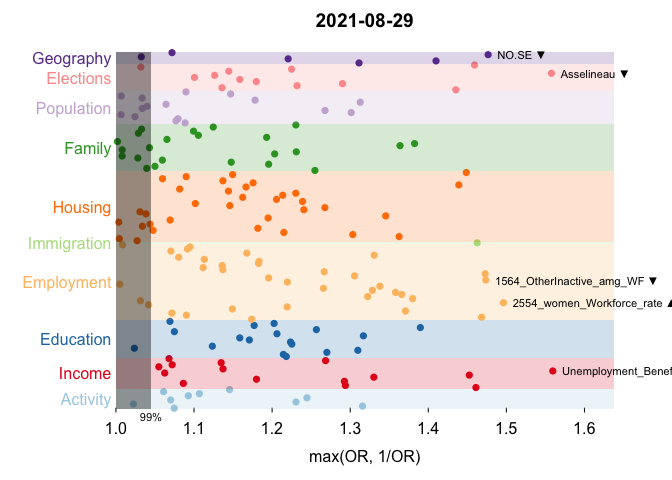
\includegraphics{vaccination-indicators_files/figure-latex/manhattan_decilesQ_withChildren-3.pdf}

\begin{verbatim}
## Warning in text.default(y = tmp$i, x = tmp$OR.abs, adj = c(0, 0.5), labels
## = paste0(" ", : conversion failure on ' Asselineau ▼' in 'mbcsToSbcs': dot
## substituted for <e2>
\end{verbatim}

\begin{verbatim}
## Warning in text.default(y = tmp$i, x = tmp$OR.abs, adj = c(0, 0.5), labels
## = paste0(" ", : conversion failure on ' Asselineau ▼' in 'mbcsToSbcs': dot
## substituted for <96>
\end{verbatim}

\begin{verbatim}
## Warning in text.default(y = tmp$i, x = tmp$OR.abs, adj = c(0, 0.5), labels
## = paste0(" ", : conversion failure on ' Asselineau ▼' in 'mbcsToSbcs': dot
## substituted for <bc>
\end{verbatim}

\begin{verbatim}
## Warning in text.default(y = tmp$i, x = tmp$OR.abs, adj = c(0, 0.5), labels =
## paste0(" ", : conversion failure on ' Unemployment_Benef ▼' in 'mbcsToSbcs':
## dot substituted for <e2>
\end{verbatim}

\begin{verbatim}
## Warning in text.default(y = tmp$i, x = tmp$OR.abs, adj = c(0, 0.5), labels =
## paste0(" ", : conversion failure on ' Unemployment_Benef ▼' in 'mbcsToSbcs':
## dot substituted for <96>
\end{verbatim}

\begin{verbatim}
## Warning in text.default(y = tmp$i, x = tmp$OR.abs, adj = c(0, 0.5), labels =
## paste0(" ", : conversion failure on ' Unemployment_Benef ▼' in 'mbcsToSbcs':
## dot substituted for <bc>
\end{verbatim}

\begin{verbatim}
## Warning in text.default(y = tmp$i, x = tmp$OR.abs, adj = c(0, 0.5), labels
## = paste0(" ", : conversion failure on ' Immigrant ▼' in 'mbcsToSbcs': dot
## substituted for <e2>
\end{verbatim}

\begin{verbatim}
## Warning in text.default(y = tmp$i, x = tmp$OR.abs, adj = c(0, 0.5), labels
## = paste0(" ", : conversion failure on ' Immigrant ▼' in 'mbcsToSbcs': dot
## substituted for <96>
\end{verbatim}

\begin{verbatim}
## Warning in text.default(y = tmp$i, x = tmp$OR.abs, adj = c(0, 0.5), labels
## = paste0(" ", : conversion failure on ' Immigrant ▼' in 'mbcsToSbcs': dot
## substituted for <bc>
\end{verbatim}

\begin{verbatim}
## Warning in text.default(y = tmp$i, x = tmp$OR.abs, adj = c(0, 0.5), labels
## = paste0(" ", : conversion failure on ' 2554_women_Workforce_rate ▲' in
## 'mbcsToSbcs': dot substituted for <e2>
\end{verbatim}

\begin{verbatim}
## Warning in text.default(y = tmp$i, x = tmp$OR.abs, adj = c(0, 0.5), labels
## = paste0(" ", : conversion failure on ' 2554_women_Workforce_rate ▲' in
## 'mbcsToSbcs': dot substituted for <96>
\end{verbatim}

\begin{verbatim}
## Warning in text.default(y = tmp$i, x = tmp$OR.abs, adj = c(0, 0.5), labels
## = paste0(" ", : conversion failure on ' 2554_women_Workforce_rate ▲' in
## 'mbcsToSbcs': dot substituted for <b2>
\end{verbatim}

\begin{verbatim}
## Warning in text.default(y = tmp$i, x = tmp$OR.abs, adj = c(0, 0.5), labels =
## paste0(" ", : conversion failure on ' Overcrowding_rate ▼' in 'mbcsToSbcs': dot
## substituted for <e2>
\end{verbatim}

\begin{verbatim}
## Warning in text.default(y = tmp$i, x = tmp$OR.abs, adj = c(0, 0.5), labels =
## paste0(" ", : conversion failure on ' Overcrowding_rate ▼' in 'mbcsToSbcs': dot
## substituted for <96>
\end{verbatim}

\begin{verbatim}
## Warning in text.default(y = tmp$i, x = tmp$OR.abs, adj = c(0, 0.5), labels =
## paste0(" ", : conversion failure on ' Overcrowding_rate ▼' in 'mbcsToSbcs': dot
## substituted for <bc>
\end{verbatim}

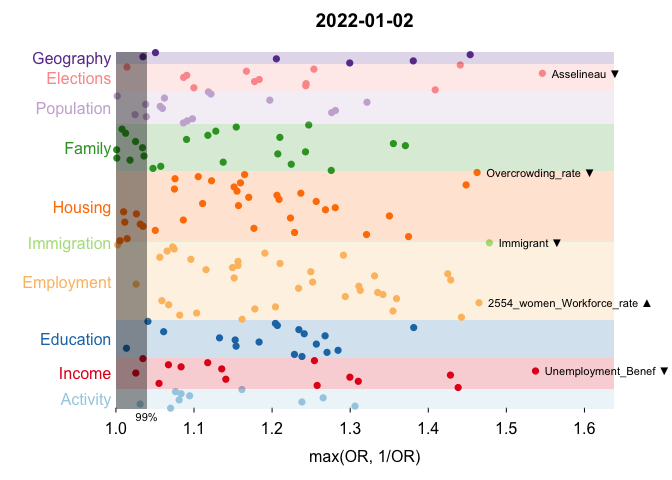
\includegraphics{vaccination-indicators_files/figure-latex/manhattan_decilesQ_withChildren-4.pdf}

\begin{Shaded}
\begin{Highlighting}[]
\NormalTok{suffix }\OtherTok{\textless{}{-}} \StringTok{".adults"}

\NormalTok{xx }\OtherTok{\textless{}{-}}\NormalTok{ outDec}
\NormalTok{xx}\SpecialCharTok{$}\NormalTok{OR }\OtherTok{\textless{}{-}}\NormalTok{ outDec[, }\FunctionTok{paste0}\NormalTok{(}\StringTok{"OR"}\NormalTok{, suffix)]}
\NormalTok{xx}\SpecialCharTok{$}\NormalTok{OR.abs }\OtherTok{\textless{}{-}}\NormalTok{ outDec[, }\FunctionTok{paste0}\NormalTok{(}\StringTok{"OR.abs"}\NormalTok{, suffix)]}
\NormalTok{xx}\SpecialCharTok{$}\NormalTok{OR.abs.CI.max }\OtherTok{\textless{}{-}}\NormalTok{ outDec[, }\FunctionTok{paste0}\NormalTok{(}\StringTok{"OR.abs"}\NormalTok{, suffix)]}

\FunctionTok{plotManhattan}\NormalTok{(xx, }\AttributeTok{ntop =} \DecValTok{5}\NormalTok{)}
\end{Highlighting}
\end{Shaded}

\begin{verbatim}
## Warning in text.default(y = tmp$i, x = tmp$OR.abs, adj = c(0, 0.5), labels
## = paste0(" ", : conversion failure on ' 1564_OtherInactive_amg_WF ▼' in
## 'mbcsToSbcs': dot substituted for <e2>
\end{verbatim}

\begin{verbatim}
## Warning in text.default(y = tmp$i, x = tmp$OR.abs, adj = c(0, 0.5), labels
## = paste0(" ", : conversion failure on ' 1564_OtherInactive_amg_WF ▼' in
## 'mbcsToSbcs': dot substituted for <96>
\end{verbatim}

\begin{verbatim}
## Warning in text.default(y = tmp$i, x = tmp$OR.abs, adj = c(0, 0.5), labels
## = paste0(" ", : conversion failure on ' 1564_OtherInactive_amg_WF ▼' in
## 'mbcsToSbcs': dot substituted for <bc>
\end{verbatim}

\begin{verbatim}
## Warning in text.default(y = tmp$i, x = tmp$OR.abs, adj = c(0, 0.5), labels
## = paste0(" ", : conversion failure on ' 1564_OtherInactive_amg_NW ▼' in
## 'mbcsToSbcs': dot substituted for <e2>
\end{verbatim}

\begin{verbatim}
## Warning in text.default(y = tmp$i, x = tmp$OR.abs, adj = c(0, 0.5), labels
## = paste0(" ", : conversion failure on ' 1564_OtherInactive_amg_NW ▼' in
## 'mbcsToSbcs': dot substituted for <96>
\end{verbatim}

\begin{verbatim}
## Warning in text.default(y = tmp$i, x = tmp$OR.abs, adj = c(0, 0.5), labels
## = paste0(" ", : conversion failure on ' 1564_OtherInactive_amg_NW ▼' in
## 'mbcsToSbcs': dot substituted for <bc>
\end{verbatim}

\begin{verbatim}
## Warning in text.default(y = tmp$i, x = tmp$OR.abs, adj = c(0, 0.5), labels =
## paste0(" ", : conversion failure on ' Unemployment_Benef ▼' in 'mbcsToSbcs':
## dot substituted for <e2>
\end{verbatim}

\begin{verbatim}
## Warning in text.default(y = tmp$i, x = tmp$OR.abs, adj = c(0, 0.5), labels =
## paste0(" ", : conversion failure on ' Unemployment_Benef ▼' in 'mbcsToSbcs':
## dot substituted for <96>
\end{verbatim}

\begin{verbatim}
## Warning in text.default(y = tmp$i, x = tmp$OR.abs, adj = c(0, 0.5), labels =
## paste0(" ", : conversion failure on ' Unemployment_Benef ▼' in 'mbcsToSbcs':
## dot substituted for <bc>
\end{verbatim}

\begin{verbatim}
## Warning in text.default(y = tmp$i, x = tmp$OR.abs, adj = c(0, 0.5), labels
## = paste0(" ", : conversion failure on ' 15._men_NoDiploma_amg_mWF ▼' in
## 'mbcsToSbcs': dot substituted for <e2>
\end{verbatim}

\begin{verbatim}
## Warning in text.default(y = tmp$i, x = tmp$OR.abs, adj = c(0, 0.5), labels
## = paste0(" ", : conversion failure on ' 15._men_NoDiploma_amg_mWF ▼' in
## 'mbcsToSbcs': dot substituted for <96>
\end{verbatim}

\begin{verbatim}
## Warning in text.default(y = tmp$i, x = tmp$OR.abs, adj = c(0, 0.5), labels
## = paste0(" ", : conversion failure on ' 15._men_NoDiploma_amg_mWF ▼' in
## 'mbcsToSbcs': dot substituted for <bc>
\end{verbatim}

\begin{verbatim}
## Warning in text.default(y = tmp$i, x = tmp$OR.abs, adj = c(0, 0.5), labels =
## paste0(" ", : conversion failure on ' Median_st_Living ▲' in 'mbcsToSbcs': dot
## substituted for <e2>
\end{verbatim}

\begin{verbatim}
## Warning in text.default(y = tmp$i, x = tmp$OR.abs, adj = c(0, 0.5), labels =
## paste0(" ", : conversion failure on ' Median_st_Living ▲' in 'mbcsToSbcs': dot
## substituted for <96>
\end{verbatim}

\begin{verbatim}
## Warning in text.default(y = tmp$i, x = tmp$OR.abs, adj = c(0, 0.5), labels =
## paste0(" ", : conversion failure on ' Median_st_Living ▲' in 'mbcsToSbcs': dot
## substituted for <b2>
\end{verbatim}

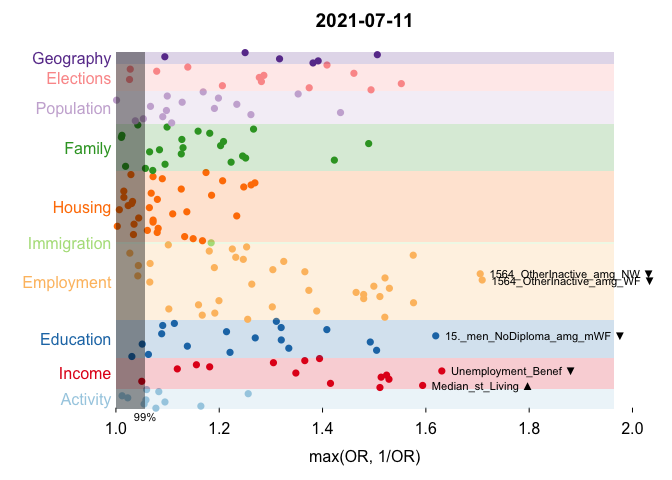
\includegraphics{vaccination-indicators_files/figure-latex/manhattan_decilesQ_adultsOnly-1.pdf}

\begin{verbatim}
## Warning in text.default(y = tmp$i, x = tmp$OR.abs, adj = c(0, 0.5), labels =
## paste0(" ", : conversion failure on ' Unemployment_Benef ▼' in 'mbcsToSbcs':
## dot substituted for <e2>
\end{verbatim}

\begin{verbatim}
## Warning in text.default(y = tmp$i, x = tmp$OR.abs, adj = c(0, 0.5), labels =
## paste0(" ", : conversion failure on ' Unemployment_Benef ▼' in 'mbcsToSbcs':
## dot substituted for <96>
\end{verbatim}

\begin{verbatim}
## Warning in text.default(y = tmp$i, x = tmp$OR.abs, adj = c(0, 0.5), labels =
## paste0(" ", : conversion failure on ' Unemployment_Benef ▼' in 'mbcsToSbcs':
## dot substituted for <bc>
\end{verbatim}

\begin{verbatim}
## Warning in text.default(y = tmp$i, x = tmp$OR.abs, adj = c(0, 0.5), labels
## = paste0(" ", : conversion failure on ' 1564_OtherInactive_amg_NW ▼' in
## 'mbcsToSbcs': dot substituted for <e2>
\end{verbatim}

\begin{verbatim}
## Warning in text.default(y = tmp$i, x = tmp$OR.abs, adj = c(0, 0.5), labels
## = paste0(" ", : conversion failure on ' 1564_OtherInactive_amg_NW ▼' in
## 'mbcsToSbcs': dot substituted for <96>
\end{verbatim}

\begin{verbatim}
## Warning in text.default(y = tmp$i, x = tmp$OR.abs, adj = c(0, 0.5), labels
## = paste0(" ", : conversion failure on ' 1564_OtherInactive_amg_NW ▼' in
## 'mbcsToSbcs': dot substituted for <bc>
\end{verbatim}

\begin{verbatim}
## Warning in text.default(y = tmp$i, x = tmp$OR.abs, adj = c(0, 0.5), labels
## = paste0(" ", : conversion failure on ' 1564_OtherInactive_amg_WF ▼' in
## 'mbcsToSbcs': dot substituted for <e2>
\end{verbatim}

\begin{verbatim}
## Warning in text.default(y = tmp$i, x = tmp$OR.abs, adj = c(0, 0.5), labels
## = paste0(" ", : conversion failure on ' 1564_OtherInactive_amg_WF ▼' in
## 'mbcsToSbcs': dot substituted for <96>
\end{verbatim}

\begin{verbatim}
## Warning in text.default(y = tmp$i, x = tmp$OR.abs, adj = c(0, 0.5), labels
## = paste0(" ", : conversion failure on ' 1564_OtherInactive_amg_WF ▼' in
## 'mbcsToSbcs': dot substituted for <bc>
\end{verbatim}

\begin{verbatim}
## Warning in text.default(y = tmp$i, x = tmp$OR.abs, adj = c(0, 0.5), labels
## = paste0(" ", : conversion failure on ' 2554_women_Workforce_rate ▲' in
## 'mbcsToSbcs': dot substituted for <e2>
\end{verbatim}

\begin{verbatim}
## Warning in text.default(y = tmp$i, x = tmp$OR.abs, adj = c(0, 0.5), labels
## = paste0(" ", : conversion failure on ' 2554_women_Workforce_rate ▲' in
## 'mbcsToSbcs': dot substituted for <96>
\end{verbatim}

\begin{verbatim}
## Warning in text.default(y = tmp$i, x = tmp$OR.abs, adj = c(0, 0.5), labels
## = paste0(" ", : conversion failure on ' 2554_women_Workforce_rate ▲' in
## 'mbcsToSbcs': dot substituted for <b2>
\end{verbatim}

\begin{verbatim}
## Warning in text.default(y = tmp$i, x = tmp$OR.abs, adj = c(0, 0.5), labels =
## paste0(" ", : conversion failure on ' NO.SE ▼' in 'mbcsToSbcs': dot substituted
## for <e2>
\end{verbatim}

\begin{verbatim}
## Warning in text.default(y = tmp$i, x = tmp$OR.abs, adj = c(0, 0.5), labels =
## paste0(" ", : conversion failure on ' NO.SE ▼' in 'mbcsToSbcs': dot substituted
## for <96>
\end{verbatim}

\begin{verbatim}
## Warning in text.default(y = tmp$i, x = tmp$OR.abs, adj = c(0, 0.5), labels =
## paste0(" ", : conversion failure on ' NO.SE ▼' in 'mbcsToSbcs': dot substituted
## for <bc>
\end{verbatim}

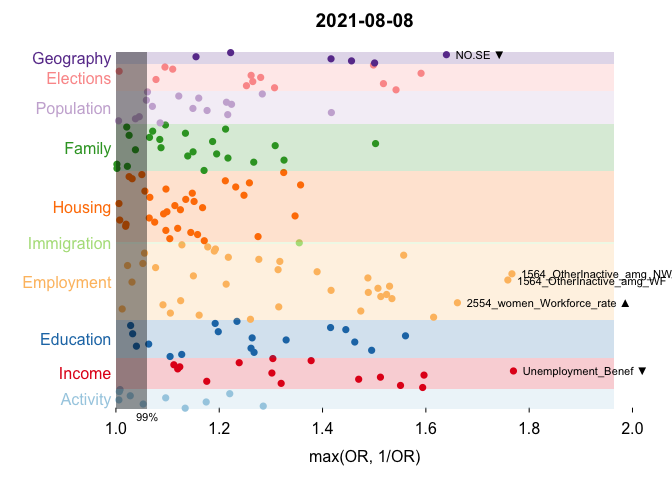
\includegraphics{vaccination-indicators_files/figure-latex/manhattan_decilesQ_adultsOnly-2.pdf}

\begin{verbatim}
## Warning in text.default(y = tmp$i, x = tmp$OR.abs, adj = c(0, 0.5), labels =
## paste0(" ", : conversion failure on ' Unemployment_Benef ▼' in 'mbcsToSbcs':
## dot substituted for <e2>
\end{verbatim}

\begin{verbatim}
## Warning in text.default(y = tmp$i, x = tmp$OR.abs, adj = c(0, 0.5), labels =
## paste0(" ", : conversion failure on ' Unemployment_Benef ▼' in 'mbcsToSbcs':
## dot substituted for <96>
\end{verbatim}

\begin{verbatim}
## Warning in text.default(y = tmp$i, x = tmp$OR.abs, adj = c(0, 0.5), labels =
## paste0(" ", : conversion failure on ' Unemployment_Benef ▼' in 'mbcsToSbcs':
## dot substituted for <bc>
\end{verbatim}

\begin{verbatim}
## Warning in text.default(y = tmp$i, x = tmp$OR.abs, adj = c(0, 0.5), labels =
## paste0(" ", : conversion failure on ' NO.SE ▼' in 'mbcsToSbcs': dot substituted
## for <e2>
\end{verbatim}

\begin{verbatim}
## Warning in text.default(y = tmp$i, x = tmp$OR.abs, adj = c(0, 0.5), labels =
## paste0(" ", : conversion failure on ' NO.SE ▼' in 'mbcsToSbcs': dot substituted
## for <96>
\end{verbatim}

\begin{verbatim}
## Warning in text.default(y = tmp$i, x = tmp$OR.abs, adj = c(0, 0.5), labels =
## paste0(" ", : conversion failure on ' NO.SE ▼' in 'mbcsToSbcs': dot substituted
## for <bc>
\end{verbatim}

\begin{verbatim}
## Warning in text.default(y = tmp$i, x = tmp$OR.abs, adj = c(0, 0.5), labels
## = paste0(" ", : conversion failure on ' 1564_OtherInactive_amg_NW ▼' in
## 'mbcsToSbcs': dot substituted for <e2>
\end{verbatim}

\begin{verbatim}
## Warning in text.default(y = tmp$i, x = tmp$OR.abs, adj = c(0, 0.5), labels
## = paste0(" ", : conversion failure on ' 1564_OtherInactive_amg_NW ▼' in
## 'mbcsToSbcs': dot substituted for <96>
\end{verbatim}

\begin{verbatim}
## Warning in text.default(y = tmp$i, x = tmp$OR.abs, adj = c(0, 0.5), labels
## = paste0(" ", : conversion failure on ' 1564_OtherInactive_amg_NW ▼' in
## 'mbcsToSbcs': dot substituted for <bc>
\end{verbatim}

\begin{verbatim}
## Warning in text.default(y = tmp$i, x = tmp$OR.abs, adj = c(0, 0.5), labels
## = paste0(" ", : conversion failure on ' Asselineau ▼' in 'mbcsToSbcs': dot
## substituted for <e2>
\end{verbatim}

\begin{verbatim}
## Warning in text.default(y = tmp$i, x = tmp$OR.abs, adj = c(0, 0.5), labels
## = paste0(" ", : conversion failure on ' Asselineau ▼' in 'mbcsToSbcs': dot
## substituted for <96>
\end{verbatim}

\begin{verbatim}
## Warning in text.default(y = tmp$i, x = tmp$OR.abs, adj = c(0, 0.5), labels
## = paste0(" ", : conversion failure on ' Asselineau ▼' in 'mbcsToSbcs': dot
## substituted for <bc>
\end{verbatim}

\begin{verbatim}
## Warning in text.default(y = tmp$i, x = tmp$OR.abs, adj = c(0, 0.5), labels
## = paste0(" ", : conversion failure on ' 1564_OtherInactive_amg_WF ▼' in
## 'mbcsToSbcs': dot substituted for <e2>
\end{verbatim}

\begin{verbatim}
## Warning in text.default(y = tmp$i, x = tmp$OR.abs, adj = c(0, 0.5), labels
## = paste0(" ", : conversion failure on ' 1564_OtherInactive_amg_WF ▼' in
## 'mbcsToSbcs': dot substituted for <96>
\end{verbatim}

\begin{verbatim}
## Warning in text.default(y = tmp$i, x = tmp$OR.abs, adj = c(0, 0.5), labels
## = paste0(" ", : conversion failure on ' 1564_OtherInactive_amg_WF ▼' in
## 'mbcsToSbcs': dot substituted for <bc>
\end{verbatim}

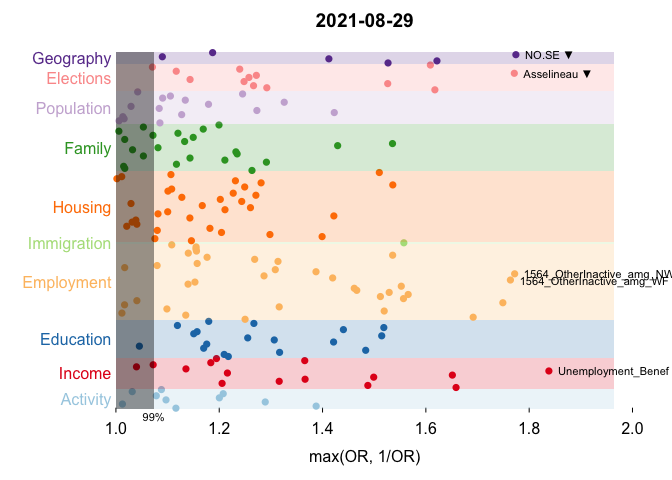
\includegraphics{vaccination-indicators_files/figure-latex/manhattan_decilesQ_adultsOnly-3.pdf}

\begin{verbatim}
## Warning in text.default(y = tmp$i, x = tmp$OR.abs, adj = c(0, 0.5), labels =
## paste0(" ", : conversion failure on ' Unemployment_Benef ▼' in 'mbcsToSbcs':
## dot substituted for <e2>
\end{verbatim}

\begin{verbatim}
## Warning in text.default(y = tmp$i, x = tmp$OR.abs, adj = c(0, 0.5), labels =
## paste0(" ", : conversion failure on ' Unemployment_Benef ▼' in 'mbcsToSbcs':
## dot substituted for <96>
\end{verbatim}

\begin{verbatim}
## Warning in text.default(y = tmp$i, x = tmp$OR.abs, adj = c(0, 0.5), labels =
## paste0(" ", : conversion failure on ' Unemployment_Benef ▼' in 'mbcsToSbcs':
## dot substituted for <bc>
\end{verbatim}

\begin{verbatim}
## Warning in text.default(y = tmp$i, x = tmp$OR.abs, adj = c(0, 0.5), labels =
## paste0(" ", : conversion failure on ' NO.SE ▼' in 'mbcsToSbcs': dot substituted
## for <e2>
\end{verbatim}

\begin{verbatim}
## Warning in text.default(y = tmp$i, x = tmp$OR.abs, adj = c(0, 0.5), labels =
## paste0(" ", : conversion failure on ' NO.SE ▼' in 'mbcsToSbcs': dot substituted
## for <96>
\end{verbatim}

\begin{verbatim}
## Warning in text.default(y = tmp$i, x = tmp$OR.abs, adj = c(0, 0.5), labels =
## paste0(" ", : conversion failure on ' NO.SE ▼' in 'mbcsToSbcs': dot substituted
## for <bc>
\end{verbatim}

\begin{verbatim}
## Warning in text.default(y = tmp$i, x = tmp$OR.abs, adj = c(0, 0.5), labels
## = paste0(" ", : conversion failure on ' Asselineau ▼' in 'mbcsToSbcs': dot
## substituted for <e2>
\end{verbatim}

\begin{verbatim}
## Warning in text.default(y = tmp$i, x = tmp$OR.abs, adj = c(0, 0.5), labels
## = paste0(" ", : conversion failure on ' Asselineau ▼' in 'mbcsToSbcs': dot
## substituted for <96>
\end{verbatim}

\begin{verbatim}
## Warning in text.default(y = tmp$i, x = tmp$OR.abs, adj = c(0, 0.5), labels
## = paste0(" ", : conversion failure on ' Asselineau ▼' in 'mbcsToSbcs': dot
## substituted for <bc>
\end{verbatim}

\begin{verbatim}
## Warning in text.default(y = tmp$i, x = tmp$OR.abs, adj = c(0, 0.5), labels
## = paste0(" ", : conversion failure on ' 1564_OtherInactive_amg_NW ▼' in
## 'mbcsToSbcs': dot substituted for <e2>
\end{verbatim}

\begin{verbatim}
## Warning in text.default(y = tmp$i, x = tmp$OR.abs, adj = c(0, 0.5), labels
## = paste0(" ", : conversion failure on ' 1564_OtherInactive_amg_NW ▼' in
## 'mbcsToSbcs': dot substituted for <96>
\end{verbatim}

\begin{verbatim}
## Warning in text.default(y = tmp$i, x = tmp$OR.abs, adj = c(0, 0.5), labels
## = paste0(" ", : conversion failure on ' 1564_OtherInactive_amg_NW ▼' in
## 'mbcsToSbcs': dot substituted for <bc>
\end{verbatim}

\begin{verbatim}
## Warning in text.default(y = tmp$i, x = tmp$OR.abs, adj = c(0, 0.5), labels
## = paste0(" ", : conversion failure on ' 1564_OtherInactive_amg_WF ▼' in
## 'mbcsToSbcs': dot substituted for <e2>
\end{verbatim}

\begin{verbatim}
## Warning in text.default(y = tmp$i, x = tmp$OR.abs, adj = c(0, 0.5), labels
## = paste0(" ", : conversion failure on ' 1564_OtherInactive_amg_WF ▼' in
## 'mbcsToSbcs': dot substituted for <96>
\end{verbatim}

\begin{verbatim}
## Warning in text.default(y = tmp$i, x = tmp$OR.abs, adj = c(0, 0.5), labels
## = paste0(" ", : conversion failure on ' 1564_OtherInactive_amg_WF ▼' in
## 'mbcsToSbcs': dot substituted for <bc>
\end{verbatim}

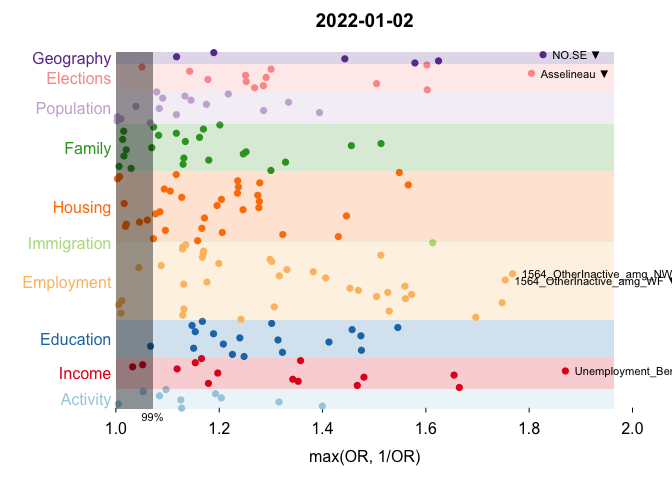
\includegraphics{vaccination-indicators_files/figure-latex/manhattan_decilesQ_adultsOnly-4.pdf}

\hypertarget{over-time}{%
\subsection{Over time}\label{over-time}}

\begin{Shaded}
\begin{Highlighting}[]
\ControlFlowTok{if}\NormalTok{(runComputations)\{}
\NormalTok{  dates }\OtherTok{\textless{}{-}} \FunctionTok{sort}\NormalTok{(}\FunctionTok{unique}\NormalTok{(vacc}\SpecialCharTok{$}\NormalTok{date))}
\NormalTok{  minDate }\OtherTok{\textless{}{-}} \StringTok{"2021{-}05{-}01"}
\NormalTok{  dates }\OtherTok{\textless{}{-}}\NormalTok{ dates[dates }\SpecialCharTok{\textgreater{}=}\NormalTok{ minDate]}
  
  \CommentTok{\# Define the combinations of parameters to be tested}
\NormalTok{  parmsTime }\OtherTok{\textless{}{-}} \FunctionTok{expand.grid}\NormalTok{(}\AttributeTok{varPred =} \FunctionTok{c}\NormalTok{(}\StringTok{"Unemployment\_Benef"}\NormalTok{, }\StringTok{"Immigrant"}\NormalTok{, }\StringTok{"Asselineau"}\NormalTok{), }
                           \AttributeTok{thedate =}\NormalTok{ dates, }
                           \AttributeTok{predTransform =} \StringTok{"discretize\_factor"}\NormalTok{, }
                           \AttributeTok{vaccAge =} \StringTok{"by\_age"}\NormalTok{, }
                           \AttributeTok{by.prbs =} \FloatTok{0.1}\NormalTok{, }
                           \AttributeTok{permutation =} \ConstantTok{FALSE}\NormalTok{,}
                           \AttributeTok{stringsAsFactors =} \ConstantTok{FALSE}\NormalTok{)}
  
  \FunctionTok{dim}\NormalTok{(parmsTime)}
  
\NormalTok{  newd }\OtherTok{\textless{}{-}} \FunctionTok{expand.grid}\NormalTok{(}\AttributeTok{age.f =} \FunctionTok{as.factor}\NormalTok{(ages), }\AttributeTok{pred.std =} \FunctionTok{as.factor}\NormalTok{(}\DecValTok{1}\SpecialCharTok{:}\DecValTok{10}\NormalTok{))}
  
  
  \CommentTok{\# Initialize output}
\NormalTok{  outC }\OtherTok{\textless{}{-}}\NormalTok{ outA }\OtherTok{\textless{}{-}} \FunctionTok{as.data.frame}\NormalTok{(}\FunctionTok{matrix}\NormalTok{(}\ConstantTok{NA}\NormalTok{, }\AttributeTok{ncol =} \DecValTok{10}\NormalTok{, }\AttributeTok{nrow =} \FunctionTok{nrow}\NormalTok{(parmsTime)))}
  
  \CommentTok{\# Compute OR for each combination of parameters}
  \ControlFlowTok{for}\NormalTok{(i }\ControlFlowTok{in} \DecValTok{1}\SpecialCharTok{:}\FunctionTok{nrow}\NormalTok{(parmsTime))\{}
    \ControlFlowTok{if}\NormalTok{(i }\SpecialCharTok{\%\%} \DecValTok{10} \SpecialCharTok{==} \DecValTok{0}\NormalTok{) }\FunctionTok{cat}\NormalTok{(i, }\StringTok{""}\NormalTok{) }\CommentTok{\# Print counter}
    \CommentTok{\# Compute the logistic regression on this combination of parameters}
\NormalTok{    mdl }\OtherTok{\textless{}{-}} \FunctionTok{do.call}\NormalTok{(getLogReg, parmsTime[i, ])}
    \CommentTok{\# Predicted values}
\NormalTok{    predsC }\OtherTok{\textless{}{-}} \FunctionTok{adjustedPredict}\NormalTok{(mdl, newd, }\AttributeTok{includeChildren =} \ConstantTok{TRUE}\NormalTok{)}
\NormalTok{    predsA }\OtherTok{\textless{}{-}} \FunctionTok{adjustedPredict}\NormalTok{(mdl, newd, }\AttributeTok{includeChildren =} \ConstantTok{FALSE}\NormalTok{)}
    
    \CommentTok{\# Save}
\NormalTok{    outC[i, ] }\OtherTok{\textless{}{-}}\NormalTok{ predsC}\SpecialCharTok{$}\NormalTok{adjustedRate}
\NormalTok{    outA[i, ] }\OtherTok{\textless{}{-}}\NormalTok{ predsA}\SpecialCharTok{$}\NormalTok{adjustedRate}
    
\NormalTok{  \}}
  
\NormalTok{  outC }\OtherTok{\textless{}{-}} \FunctionTok{cbind}\NormalTok{(parmsTime, outC)}
\NormalTok{  outA }\OtherTok{\textless{}{-}} \FunctionTok{cbind}\NormalTok{(parmsTime, outA)}
  
  \FunctionTok{save}\NormalTok{(outC, outA, dates, }\AttributeTok{file =} \StringTok{"outTime.RData"}\NormalTok{)}

\NormalTok{\}}
\end{Highlighting}
\end{Shaded}

\begin{Shaded}
\begin{Highlighting}[]
\FunctionTok{load}\NormalTok{(}\StringTok{"outTime.RData"}\NormalTok{)}

\FunctionTok{plotPropTime}\NormalTok{(outC)}
\end{Highlighting}
\end{Shaded}

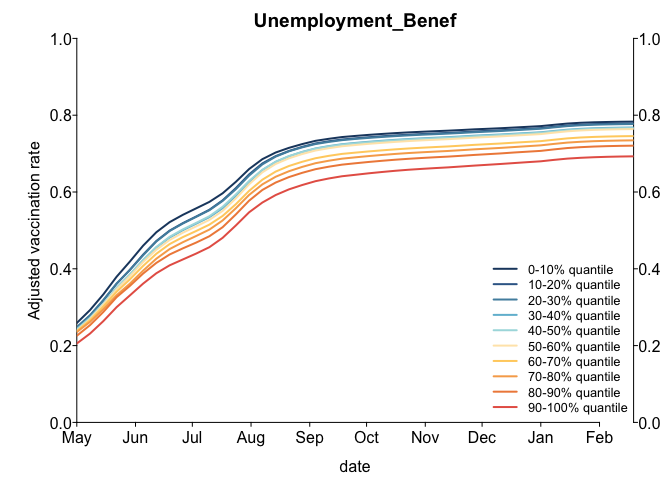
\includegraphics{vaccination-indicators_files/figure-latex/overtime_withChildren-1.pdf}
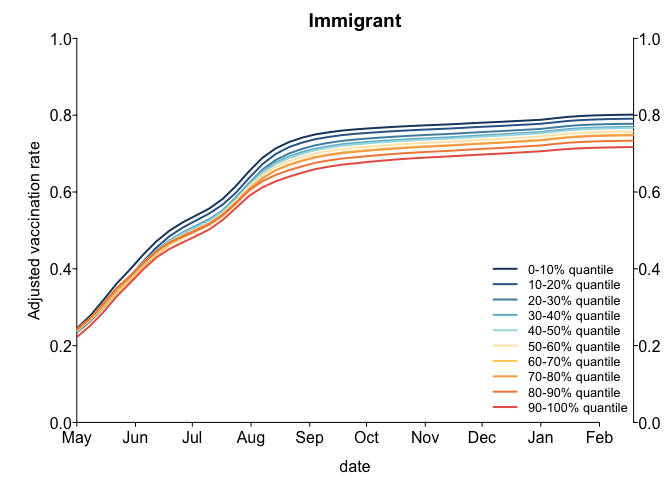
\includegraphics{vaccination-indicators_files/figure-latex/overtime_withChildren-2.pdf}
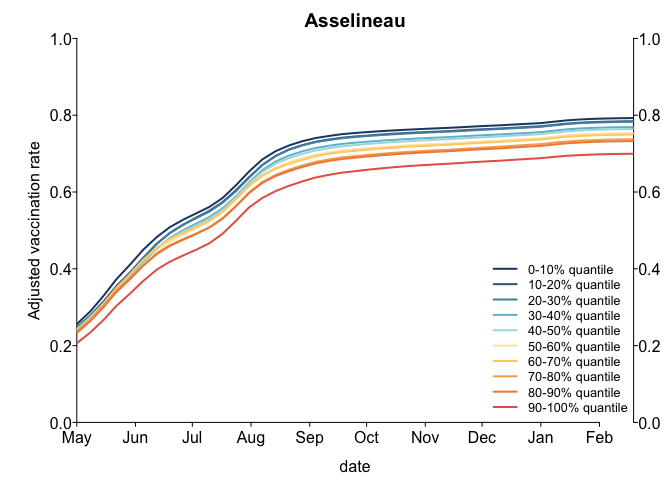
\includegraphics{vaccination-indicators_files/figure-latex/overtime_withChildren-3.pdf}

\begin{Shaded}
\begin{Highlighting}[]
\FunctionTok{plotPropTime}\NormalTok{(outA)}
\end{Highlighting}
\end{Shaded}

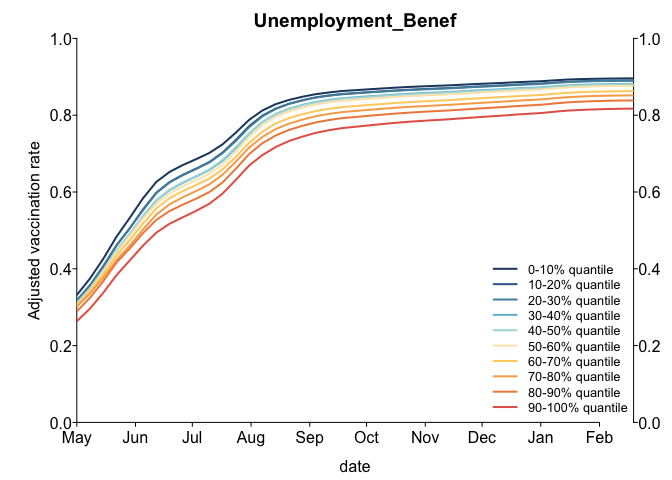
\includegraphics{vaccination-indicators_files/figure-latex/overtime_adultsOnly-1.pdf}
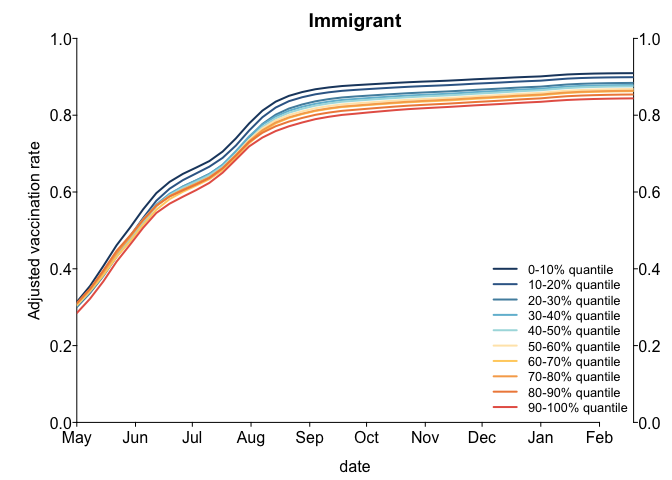
\includegraphics{vaccination-indicators_files/figure-latex/overtime_adultsOnly-2.pdf}
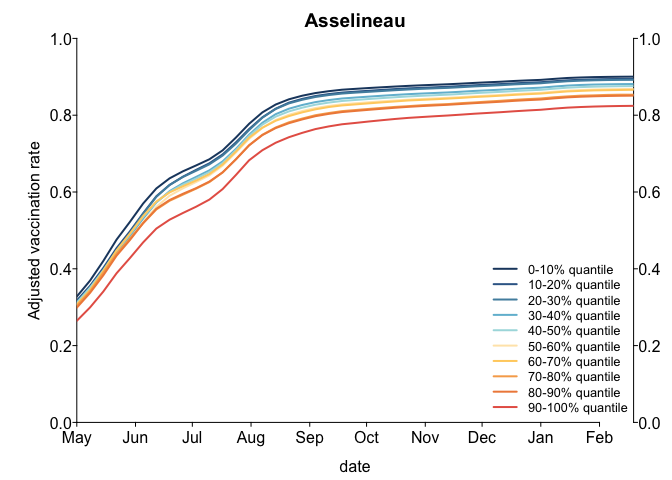
\includegraphics{vaccination-indicators_files/figure-latex/overtime_adultsOnly-3.pdf}

\hypertarget{geographic}{%
\section{Geographic}\label{geographic}}

\begin{Shaded}
\begin{Highlighting}[]
\FunctionTok{library}\NormalTok{(mapsf)}
\end{Highlighting}
\end{Shaded}

\begin{verbatim}
## Loading required package: sf
\end{verbatim}

\begin{verbatim}
## Linking to GEOS 3.9.1, GDAL 3.3.1, PROJ 8.1.0
\end{verbatim}

\begin{Shaded}
\begin{Highlighting}[]
\CommentTok{\# Geographic information for maps}
\FunctionTok{load}\NormalTok{(}\StringTok{"../data/mapFiles\_withDepReg.RData"}\NormalTok{)}
\FunctionTok{load}\NormalTok{(}\StringTok{"../data/chefslieux.RData"}\NormalTok{)}
\end{Highlighting}
\end{Shaded}

\begin{Shaded}
\begin{Highlighting}[]
\CommentTok{\#varPred \textless{}{-} "X1564\_OtherInactive\_amg\_NW"}

\FunctionTok{source}\NormalTok{(}\StringTok{"2\_plot{-}map.R"}\NormalTok{)}
\FunctionTok{plotMapVar}\NormalTok{(}\StringTok{"Unemployment\_Benef"}\NormalTok{, }\AttributeTok{byp =} \FloatTok{0.1}\NormalTok{)}
\end{Highlighting}
\end{Shaded}

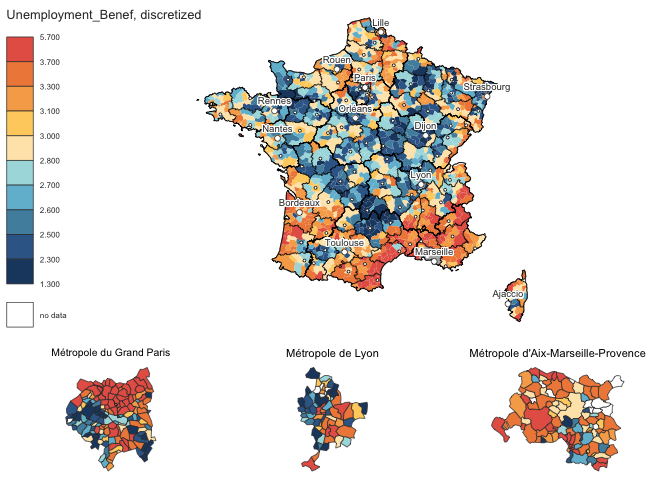
\includegraphics{vaccination-indicators_files/figure-latex/unnamed-chunk-9-1.pdf}

\begin{Shaded}
\begin{Highlighting}[]
\FunctionTok{plotMapVar}\NormalTok{(}\StringTok{"Unemployment\_Benef"}\NormalTok{, }\AttributeTok{byp =} \FloatTok{0.5}\NormalTok{)}
\end{Highlighting}
\end{Shaded}

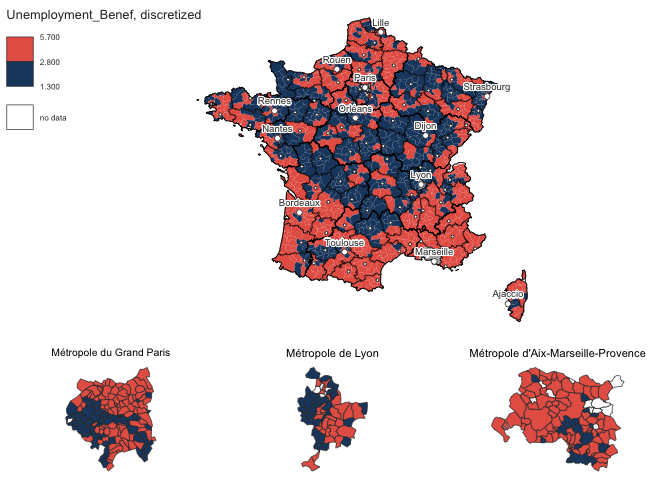
\includegraphics{vaccination-indicators_files/figure-latex/unnamed-chunk-10-1.pdf}

\begin{Shaded}
\begin{Highlighting}[]
\FunctionTok{plotMapVar}\NormalTok{(}\StringTok{"Unemployment\_Benef"}\NormalTok{, }\AttributeTok{byp =} \FloatTok{0.1}\NormalTok{)}
\end{Highlighting}
\end{Shaded}

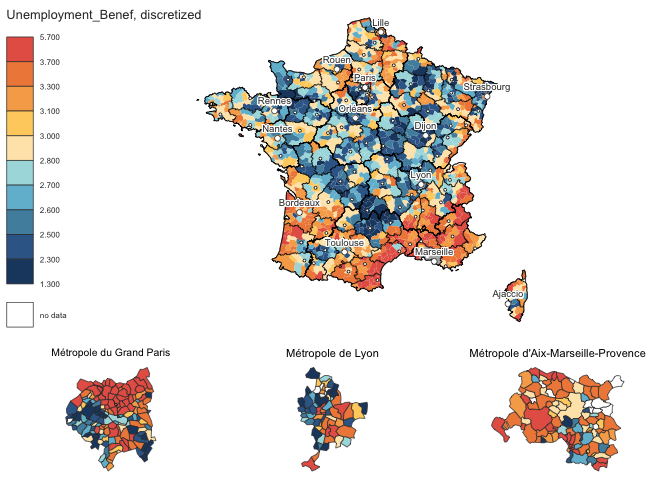
\includegraphics{vaccination-indicators_files/figure-latex/unnamed-chunk-10-2.pdf}

\begin{Shaded}
\begin{Highlighting}[]
\NormalTok{vv }\OtherTok{\textless{}{-}}\NormalTok{ dat.all[, }\StringTok{"Unemployment\_Benef"}\NormalTok{]}
\FunctionTok{plot}\NormalTok{(}\FunctionTok{discretizeQ}\NormalTok{(vv, }\FunctionTok{seq}\NormalTok{(}\DecValTok{0}\NormalTok{, }\DecValTok{1}\NormalTok{, }\FloatTok{0.1}\NormalTok{)), }
     \FunctionTok{discretizeQ}\NormalTok{(vv, }\FunctionTok{seq}\NormalTok{(}\DecValTok{0}\NormalTok{, }\DecValTok{1}\NormalTok{, }\FloatTok{0.5}\NormalTok{)))}
\end{Highlighting}
\end{Shaded}

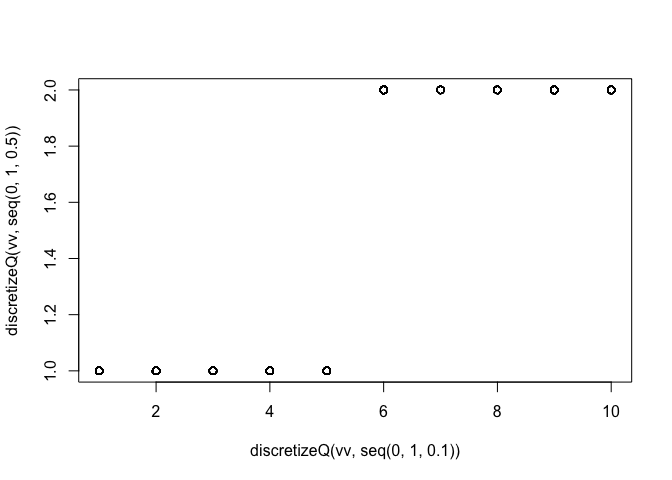
\includegraphics{vaccination-indicators_files/figure-latex/unnamed-chunk-10-3.pdf}

\begin{Shaded}
\begin{Highlighting}[]
\FunctionTok{plotMapVar}\NormalTok{(}\StringTok{"Asselineau"}\NormalTok{, }\AttributeTok{byp =} \FloatTok{0.1}\NormalTok{)}
\end{Highlighting}
\end{Shaded}

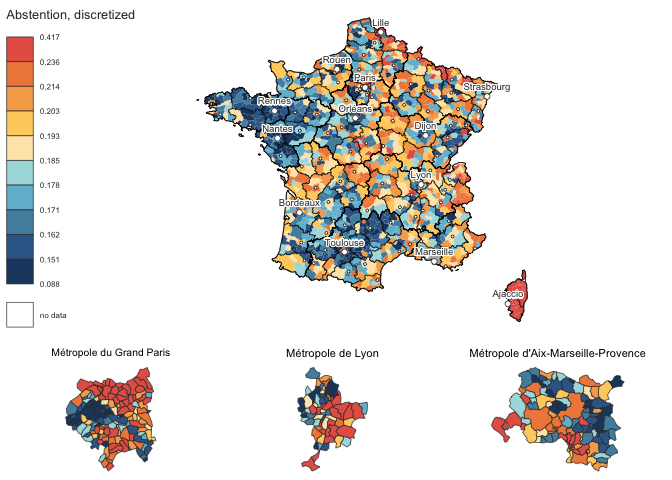
\includegraphics{vaccination-indicators_files/figure-latex/unnamed-chunk-10-4.pdf}

\begin{Shaded}
\begin{Highlighting}[]
\FunctionTok{plotMapVar}\NormalTok{(}\StringTok{"Abstention"}\NormalTok{, }\AttributeTok{byp =} \FloatTok{0.1}\NormalTok{)}
\end{Highlighting}
\end{Shaded}

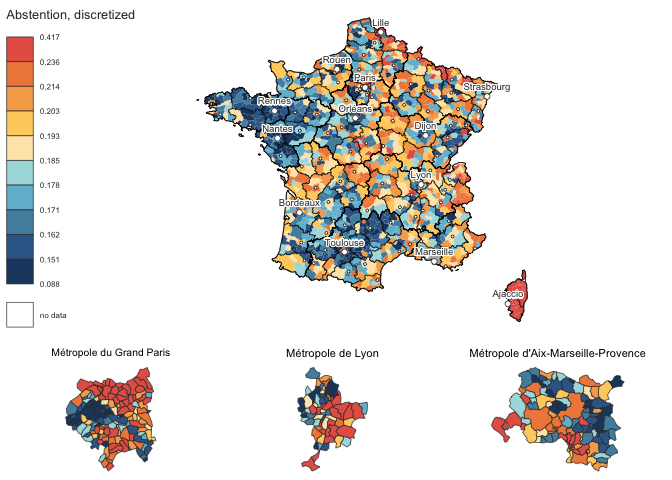
\includegraphics{vaccination-indicators_files/figure-latex/unnamed-chunk-10-5.pdf}

\begin{Shaded}
\begin{Highlighting}[]
\FunctionTok{plotMapVar}\NormalTok{(}\StringTok{"Immigrant"}\NormalTok{, }\AttributeTok{byp =} \FloatTok{0.1}\NormalTok{)}
\end{Highlighting}
\end{Shaded}

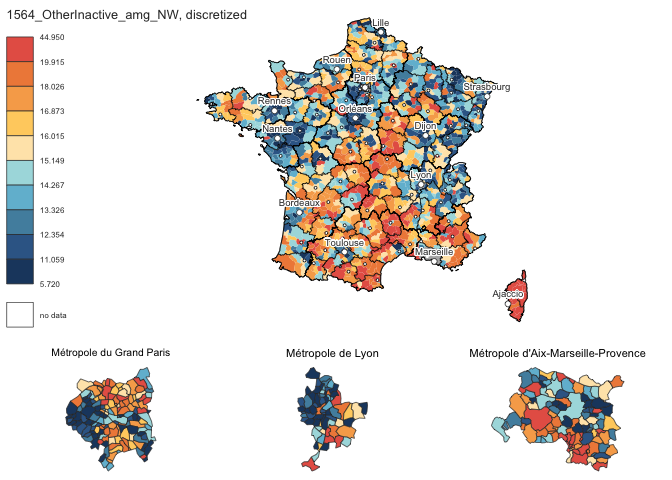
\includegraphics{vaccination-indicators_files/figure-latex/unnamed-chunk-10-6.pdf}

\begin{Shaded}
\begin{Highlighting}[]
\FunctionTok{plotMapVar}\NormalTok{(}\StringTok{"X1564\_OtherInactive\_amg\_NW"}\NormalTok{, }\AttributeTok{byp =} \FloatTok{0.1}\NormalTok{)}
\end{Highlighting}
\end{Shaded}

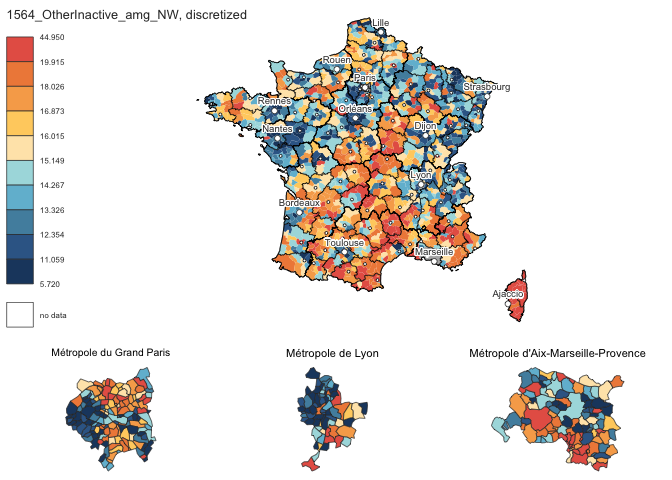
\includegraphics{vaccination-indicators_files/figure-latex/unnamed-chunk-10-7.pdf}

\hypertarget{essais}{%
\section{Essais}\label{essais}}

\begin{Shaded}
\begin{Highlighting}[]
\NormalTok{v }\OtherTok{\textless{}{-}}\NormalTok{ dat.all[, }\FunctionTok{c}\NormalTok{(}\StringTok{"codgeo"}\NormalTok{, }\StringTok{"French\_nlty"}\NormalTok{)]}
\NormalTok{vx }\OtherTok{\textless{}{-}}\NormalTok{ v[}\FunctionTok{which}\NormalTok{(}\FunctionTok{is.na}\NormalTok{(v}\SpecialCharTok{$}\NormalTok{French\_nlty)), ]}
\NormalTok{vx}
\NormalTok{v[}\DecValTok{1}\NormalTok{, ]}
\FunctionTok{head}\NormalTok{(v)}
\FunctionTok{tail}\NormalTok{(v)}

\FunctionTok{library}\NormalTok{(inseeLocalData)}
\NormalTok{?inseeLocalData}

\CommentTok{\#install.packages("insee")}
\FunctionTok{library}\NormalTok{(insee)}

\FunctionTok{get\_dataset\_list}\NormalTok{()}

\NormalTok{https}\SpecialCharTok{:}\ErrorTok{//}\NormalTok{api.insee.fr}\SpecialCharTok{/}\NormalTok{donnees}\SpecialCharTok{{-}}\NormalTok{locales}\SpecialCharTok{/}\NormalTok{V0}\FloatTok{.1}\SpecialCharTok{/}\NormalTok{donnees}\SpecialCharTok{/}\NormalTok{geo}\SpecialCharTok{{-}}\NormalTok{POP}\SpecialCharTok{@}\NormalTok{GEO2021RP2018}\SpecialCharTok{/}\NormalTok{EPCI}\FloatTok{{-}247100647.}\NormalTok{INATC}
\end{Highlighting}
\end{Shaded}

\begin{Shaded}
\begin{Highlighting}[]
\NormalTok{?prcomp}

\CommentTok{\# Predictors}
\CommentTok{\# New dataset with the predictors}
\NormalTok{dat2 }\OtherTok{\textless{}{-}}\NormalTok{ dat.nocorr[, }\SpecialCharTok{{-}}\DecValTok{1}\NormalTok{]}

\CommentTok{\# For each predictor}
\ControlFlowTok{for}\NormalTok{(col }\ControlFlowTok{in} \FunctionTok{colnames}\NormalTok{(dat2))\{}
  \CommentTok{\# Get the subset of the data}
\NormalTok{  v }\OtherTok{\textless{}{-}}\NormalTok{ dat2[, col]}
  \CommentTok{\# Compute the mean value, excluding NAs}
\NormalTok{  mv }\OtherTok{\textless{}{-}} \FunctionTok{mean}\NormalTok{(v, }\AttributeTok{na.rm =} \ConstantTok{TRUE}\NormalTok{)}
  \CommentTok{\# Fill in NAs with the mean}
\NormalTok{  v[}\FunctionTok{is.na}\NormalTok{(v)] }\OtherTok{\textless{}{-}}\NormalTok{ mv}
  \CommentTok{\# Put back in the table}
\NormalTok{  dat2[, col] }\OtherTok{\textless{}{-}}\NormalTok{ v}
\NormalTok{\}}

\NormalTok{pca }\OtherTok{\textless{}{-}} \FunctionTok{prcomp}\NormalTok{(dat2, }\AttributeTok{center =} \ConstantTok{TRUE}\NormalTok{, }\AttributeTok{scale =} \ConstantTok{TRUE}\NormalTok{)}
\FunctionTok{ggbiplot}\NormalTok{(pca)}

\FunctionTok{head}\NormalTok{(pca)}

\FunctionTok{library}\NormalTok{(devtools)}
\FunctionTok{install\_github}\NormalTok{(}\StringTok{"vqv/ggbiplot"}\NormalTok{)}
\FunctionTok{library}\NormalTok{(ggbiplot)}

\FunctionTok{plot}\NormalTok{(pca}\SpecialCharTok{$}\NormalTok{x[, }\FunctionTok{c}\NormalTok{(}\StringTok{"PC1"}\NormalTok{, }\StringTok{"PC2"}\NormalTok{)])}

\NormalTok{pcax }\OtherTok{\textless{}{-}} \FunctionTok{as.data.frame}\NormalTok{(pca}\SpecialCharTok{$}\NormalTok{x)}
\NormalTok{pcax}\SpecialCharTok{$}\NormalTok{codgeo }\OtherTok{\textless{}{-}}\NormalTok{ dat.nocorr}\SpecialCharTok{$}\NormalTok{codgeo}

\NormalTok{thedate }\OtherTok{\textless{}{-}}\NormalTok{ date3}
\NormalTok{sub }\OtherTok{\textless{}{-}}\NormalTok{ vacc[}\FunctionTok{which}\NormalTok{(vacc}\SpecialCharTok{$}\NormalTok{date }\SpecialCharTok{==}\NormalTok{ thedate }\SpecialCharTok{\&}\NormalTok{ vacc}\SpecialCharTok{$}\NormalTok{classe\_age }\SpecialCharTok{!=} \StringTok{"TOUT\_AGE"}\NormalTok{), ]}
\NormalTok{subb }\OtherTok{\textless{}{-}} \FunctionTok{adultVacc}\NormalTok{(sub)}

\NormalTok{sub3 }\OtherTok{\textless{}{-}} \FunctionTok{merge}\NormalTok{(subb, pcax, }\AttributeTok{all =} \ConstantTok{TRUE}\NormalTok{, }\AttributeTok{by =} \StringTok{"codgeo"}\NormalTok{)}
\NormalTok{sub3}\SpecialCharTok{$}\NormalTok{typeTaux }\OtherTok{\textless{}{-}} \FunctionTok{discretizeQ}\NormalTok{(sub3}\SpecialCharTok{$}\NormalTok{taux\_cumu, }\AttributeTok{prbs =} \FunctionTok{seq}\NormalTok{(}\DecValTok{0}\NormalTok{, }\DecValTok{1}\NormalTok{, }\AttributeTok{by =} \FloatTok{0.1}\NormalTok{))}
\NormalTok{palCat }\OtherTok{\textless{}{-}} \FunctionTok{rev}\NormalTok{(}\FunctionTok{met.brewer}\NormalTok{(}\StringTok{"Hiroshige"}\NormalTok{, }\AttributeTok{n =} \DecValTok{10}\NormalTok{, }\AttributeTok{type =} \StringTok{"continuous"}\NormalTok{))}
\FunctionTok{names}\NormalTok{(palCat) }\OtherTok{\textless{}{-}} \DecValTok{1}\SpecialCharTok{:}\DecValTok{10}

\FunctionTok{plot}\NormalTok{(sub3}\SpecialCharTok{$}\NormalTok{PC1, sub3}\SpecialCharTok{$}\NormalTok{PC2, }\AttributeTok{col =}\NormalTok{ palCat[sub3}\SpecialCharTok{$}\NormalTok{typeTaux], }\AttributeTok{pch =} \DecValTok{16}\NormalTok{)}

\FunctionTok{str}\NormalTok{(pca)}
\FunctionTok{head}\NormalTok{(sub3)}
\FunctionTok{dim}\NormalTok{(subb)}
\FunctionTok{dim}\NormalTok{(pcax)  }

\FunctionTok{sort}\NormalTok{(pca}\SpecialCharTok{$}\NormalTok{rotation[, }\StringTok{"PC1"}\NormalTok{], }\AttributeTok{decreasing =} \ConstantTok{TRUE}\NormalTok{)[}\DecValTok{1}\SpecialCharTok{:}\DecValTok{30}\NormalTok{]}
\FunctionTok{sort}\NormalTok{(pca}\SpecialCharTok{$}\NormalTok{rotation[, }\StringTok{"PC2"}\NormalTok{], }\AttributeTok{decreasing =} \ConstantTok{TRUE}\NormalTok{)[}\DecValTok{1}\SpecialCharTok{:}\DecValTok{30}\NormalTok{]}

\FunctionTok{head}\NormalTok{(pca)}
\FunctionTok{summary}\NormalTok{(pca)}

\NormalTok{pca}\SpecialCharTok{$}\NormalTok{sdev }\SpecialCharTok{/} \FunctionTok{sum}\NormalTok{(pca}\SpecialCharTok{$}\NormalTok{sdev)}
\FunctionTok{str}\NormalTok{(pca)}

\FunctionTok{length}\NormalTok{(pca}\SpecialCharTok{$}\NormalTok{rotation[, }\StringTok{"PC2"}\NormalTok{])}
\FunctionTok{length}\NormalTok{(subb}\SpecialCharTok{$}\NormalTok{taux\_cumu)}

\FunctionTok{plot}\NormalTok{(sub3}\SpecialCharTok{$}\NormalTok{PC2, sub3}\SpecialCharTok{$}\NormalTok{taux\_cumu)}

\NormalTok{out }\OtherTok{\textless{}{-}} \FunctionTok{matrix}\NormalTok{(}\ConstantTok{NA}\NormalTok{, }\AttributeTok{nrow =}\NormalTok{ (}\FunctionTok{ncol}\NormalTok{(pcax) }\SpecialCharTok{{-}} \DecValTok{1}\NormalTok{), }\AttributeTok{ncol =} \DecValTok{4}\NormalTok{)}
\ControlFlowTok{for}\NormalTok{(i }\ControlFlowTok{in} \DecValTok{1}\SpecialCharTok{:}\NormalTok{(}\FunctionTok{ncol}\NormalTok{(pcax) }\SpecialCharTok{{-}} \DecValTok{1}\NormalTok{))\{}
\NormalTok{  mdl }\OtherTok{\textless{}{-}} \FunctionTok{cor.test}\NormalTok{(sub3[, }\FunctionTok{paste0}\NormalTok{(}\StringTok{"PC"}\NormalTok{, i)], sub3}\SpecialCharTok{$}\NormalTok{taux\_cumu)}
\NormalTok{  out[i, ] }\OtherTok{\textless{}{-}} \FunctionTok{c}\NormalTok{(mdl}\SpecialCharTok{$}\NormalTok{estimate, mdl}\SpecialCharTok{$}\NormalTok{conf.int, mdl}\SpecialCharTok{$}\NormalTok{p.value)}
\NormalTok{\}}
\NormalTok{out }\OtherTok{\textless{}{-}} \FunctionTok{as.data.frame}\NormalTok{(out)}
\FunctionTok{names}\NormalTok{(out) }\OtherTok{\textless{}{-}} \FunctionTok{c}\NormalTok{(}\StringTok{"estimate"}\NormalTok{, }\StringTok{"ci1"}\NormalTok{, }\StringTok{"ci2"}\NormalTok{, }\StringTok{"pval"}\NormalTok{)}
\NormalTok{out}\SpecialCharTok{$}\NormalTok{PC }\OtherTok{\textless{}{-}} \FunctionTok{seq\_len}\NormalTok{(}\FunctionTok{nrow}\NormalTok{(out))}

\NormalTok{out[}\FunctionTok{order}\NormalTok{(}\FunctionTok{abs}\NormalTok{(out}\SpecialCharTok{$}\NormalTok{estimate), }\AttributeTok{decreasing =} \ConstantTok{TRUE}\NormalTok{), ][}\DecValTok{1}\SpecialCharTok{:}\DecValTok{5}\NormalTok{, ]}
\NormalTok{ii }\OtherTok{\textless{}{-}}\NormalTok{ out[}\FunctionTok{order}\NormalTok{(}\FunctionTok{abs}\NormalTok{(out}\SpecialCharTok{$}\NormalTok{estimate), }\AttributeTok{decreasing =} \ConstantTok{TRUE}\NormalTok{), ][}\DecValTok{1}\SpecialCharTok{:}\DecValTok{5}\NormalTok{, }\StringTok{"PC"}\NormalTok{]}

\CommentTok{\# Composition of the PCs}
\ControlFlowTok{for}\NormalTok{(i }\ControlFlowTok{in}\NormalTok{ ii)\{}
  \FunctionTok{print}\NormalTok{(i)}
  \FunctionTok{print}\NormalTok{(}\FunctionTok{t}\NormalTok{(}\FunctionTok{sort}\NormalTok{(pca}\SpecialCharTok{$}\NormalTok{rotation[, }\FunctionTok{paste0}\NormalTok{(}\StringTok{"PC"}\NormalTok{, i)], }\AttributeTok{decreasing =} \ConstantTok{TRUE}\NormalTok{)[}\DecValTok{1}\SpecialCharTok{:}\DecValTok{20}\NormalTok{])) }
\NormalTok{\}}
\FunctionTok{sort}\NormalTok{(pca}\SpecialCharTok{$}\NormalTok{rotation[, }\StringTok{"PC2"}\NormalTok{], }\AttributeTok{decreasing =} \ConstantTok{TRUE}\NormalTok{)[}\DecValTok{1}\SpecialCharTok{:}\DecValTok{30}\NormalTok{]}

\FunctionTok{plot}\NormalTok{(}\FunctionTok{sort}\NormalTok{(}\FunctionTok{abs}\NormalTok{(out}\SpecialCharTok{$}\NormalTok{estimate)))}

\FunctionTok{range}\NormalTok{(out}\SpecialCharTok{$}\NormalTok{estimate)}

\FunctionTok{head}\NormalTok{(out)}
\NormalTok{mdl2 }\OtherTok{\textless{}{-}} \FunctionTok{cor.test}\NormalTok{(sub3}\SpecialCharTok{$}\NormalTok{PC2, sub3}\SpecialCharTok{$}\NormalTok{taux\_cumu)}
\NormalTok{mdl2}

\NormalTok{mdl1 }\OtherTok{\textless{}{-}} \FunctionTok{cor.test}\NormalTok{(sub3}\SpecialCharTok{$}\NormalTok{PC1, sub3}\SpecialCharTok{$}\NormalTok{taux\_cumu)}
\NormalTok{mdl1}
\FunctionTok{str}\NormalTok{(mdl1)}
\FunctionTok{summary}\NormalTok{(mdl1)}
\NormalTok{mdl3 }\OtherTok{\textless{}{-}} \FunctionTok{cor.test}\NormalTok{(sub3}\SpecialCharTok{$}\NormalTok{PC3, sub3}\SpecialCharTok{$}\NormalTok{taux\_cumu)}
\NormalTok{mdl3}

\FunctionTok{summary}\NormalTok{(mdl)}

\FunctionTok{library}\NormalTok{(nlme)}
\NormalTok{?gls}
         \FunctionTok{gls}\NormalTok{(divspe }\SpecialCharTok{\textasciitilde{}}\NormalTok{ loggrad\_urb}\SpecialCharTok{+}\NormalTok{grad\_agrimean, }\AttributeTok{method =} \StringTok{"ML"}\NormalTok{, }
\AttributeTok{corr=}\FunctionTok{corExp}\NormalTok{(}\FunctionTok{c}\NormalTok{(}\DecValTok{300000}\NormalTok{,}\FloatTok{0.7}\NormalTok{), }\AttributeTok{form=}\SpecialCharTok{\textasciitilde{}}\NormalTok{x\_lambert93}\SpecialCharTok{+}\NormalTok{y\_lambert93, }\AttributeTok{nugget=}\NormalTok{T), }
\AttributeTok{na.action =}\NormalTok{ na.omit, }\AttributeTok{data =}\NormalTok{ df)}
\end{Highlighting}
\end{Shaded}


\end{document}
